% Supplementary / Extended Data Figures for Yang et al. Science 2024
% Chapter: Selection of experience for memory by hippocampal sharp wave ripples

\section*{Extended Data Figures}

\begin{figure}[htbp]
\centering
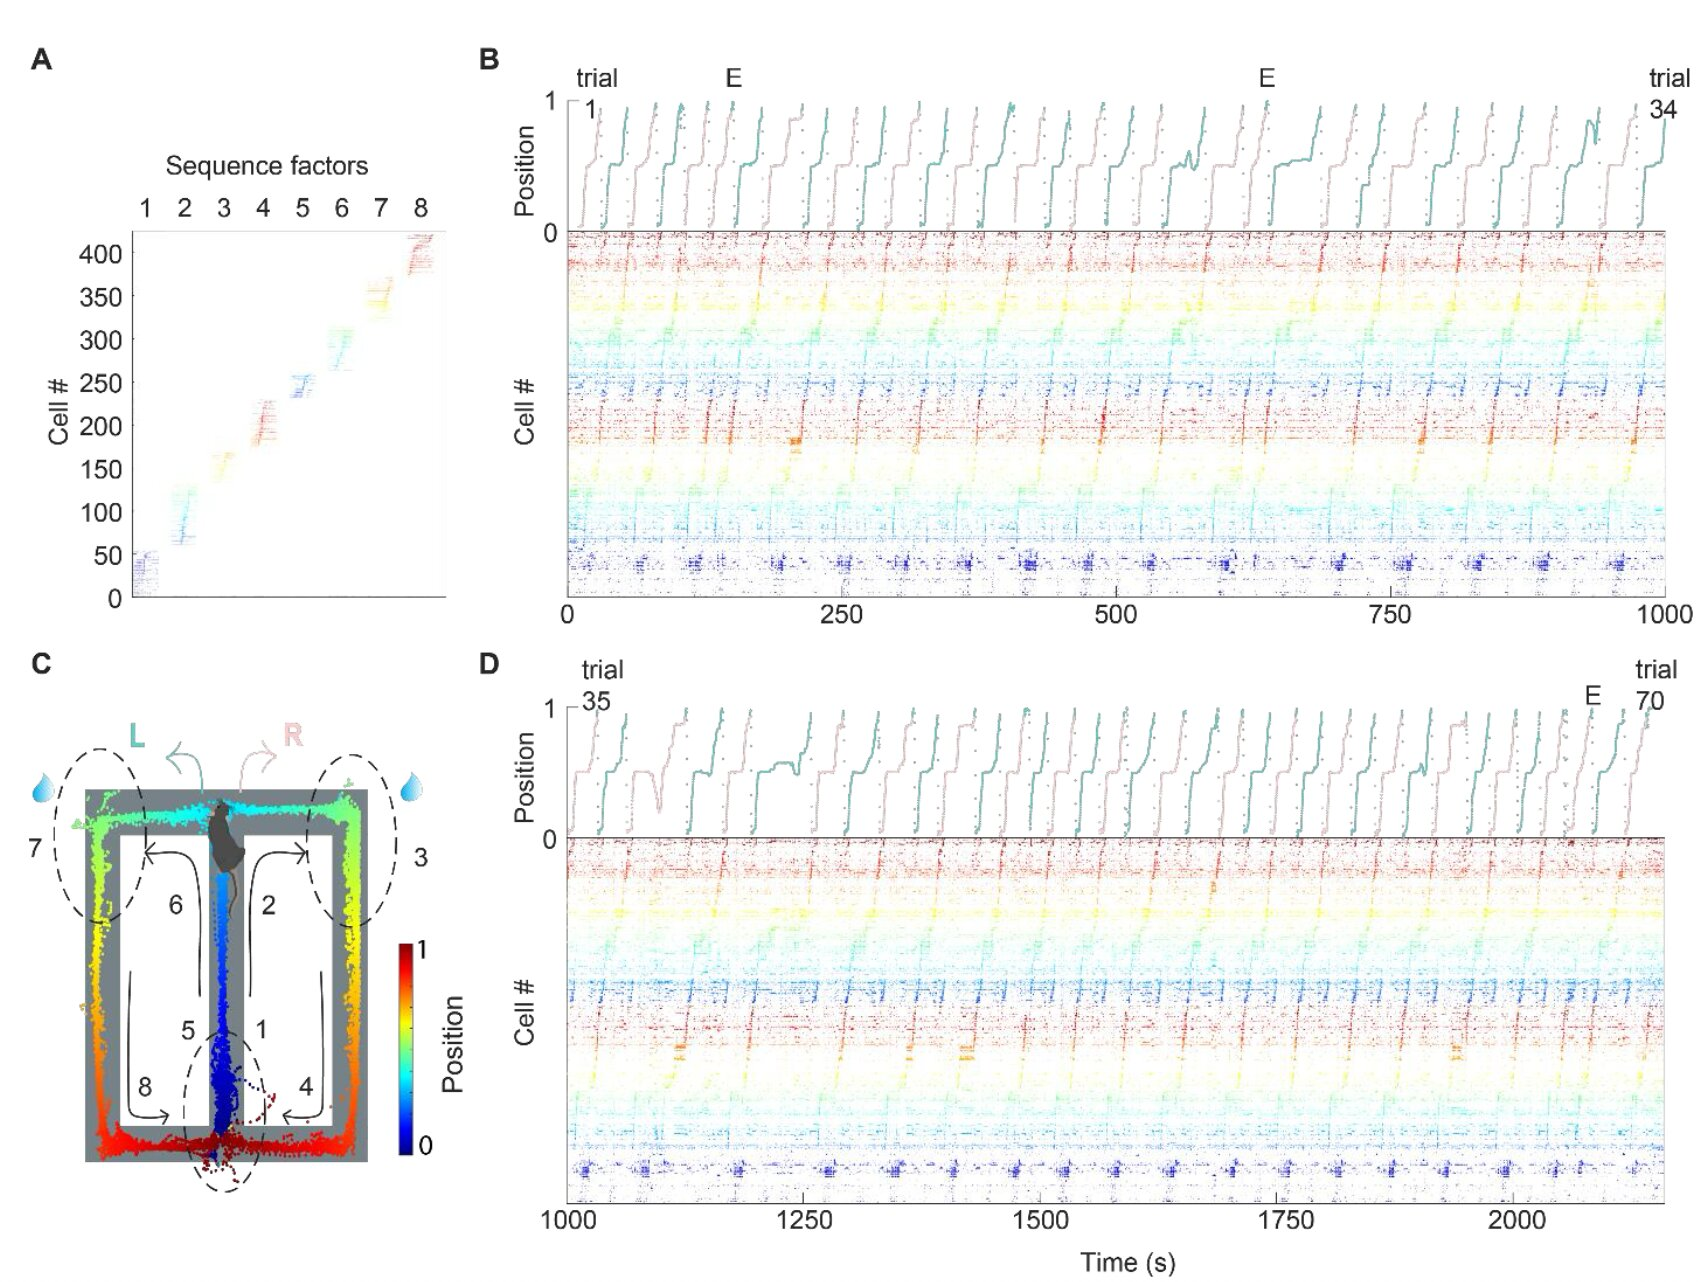
\includegraphics[width=\textwidth]{figures/ch_selection2024/Extended_Fig1.jpg}
\caption[Extended Data Fig.~1: Neural spiking data of the entire example session sorted by seqNMF]{\textbf{Extended Data Fig.~1: Neural spiking data of the entire example session sorted by seqNMF.}
(A) Eight sequence factors identified by seqNMF.
(B) Trials 1--34 (out of 70 trials in total) during the figure-eight maze task. Top, linearized position of the animal. Red, right traversal; green, left traversal. Bottom, raster plot of spiking data of 422 pyramidal cells simultaneously recorded from the right dorsal CA1 region, sorted by seqNMF, and color-coded according to the linearized position.
(C) Figure-eight maze task, where the mouse alternates between left and right arms to gain water reward (blue droplets). Animal's trajectory in the maze was colored by its linearized position. Numbers 1 to 8 indicate the mapping of the 8 seqNMF sequence factors onto the corresponding segments of the maze.
(D) Trials 35--70 of the same session as in (B).}
\label{fig:selection2024-ext1}
\end{figure}

\begin{figure}[htbp]
\centering
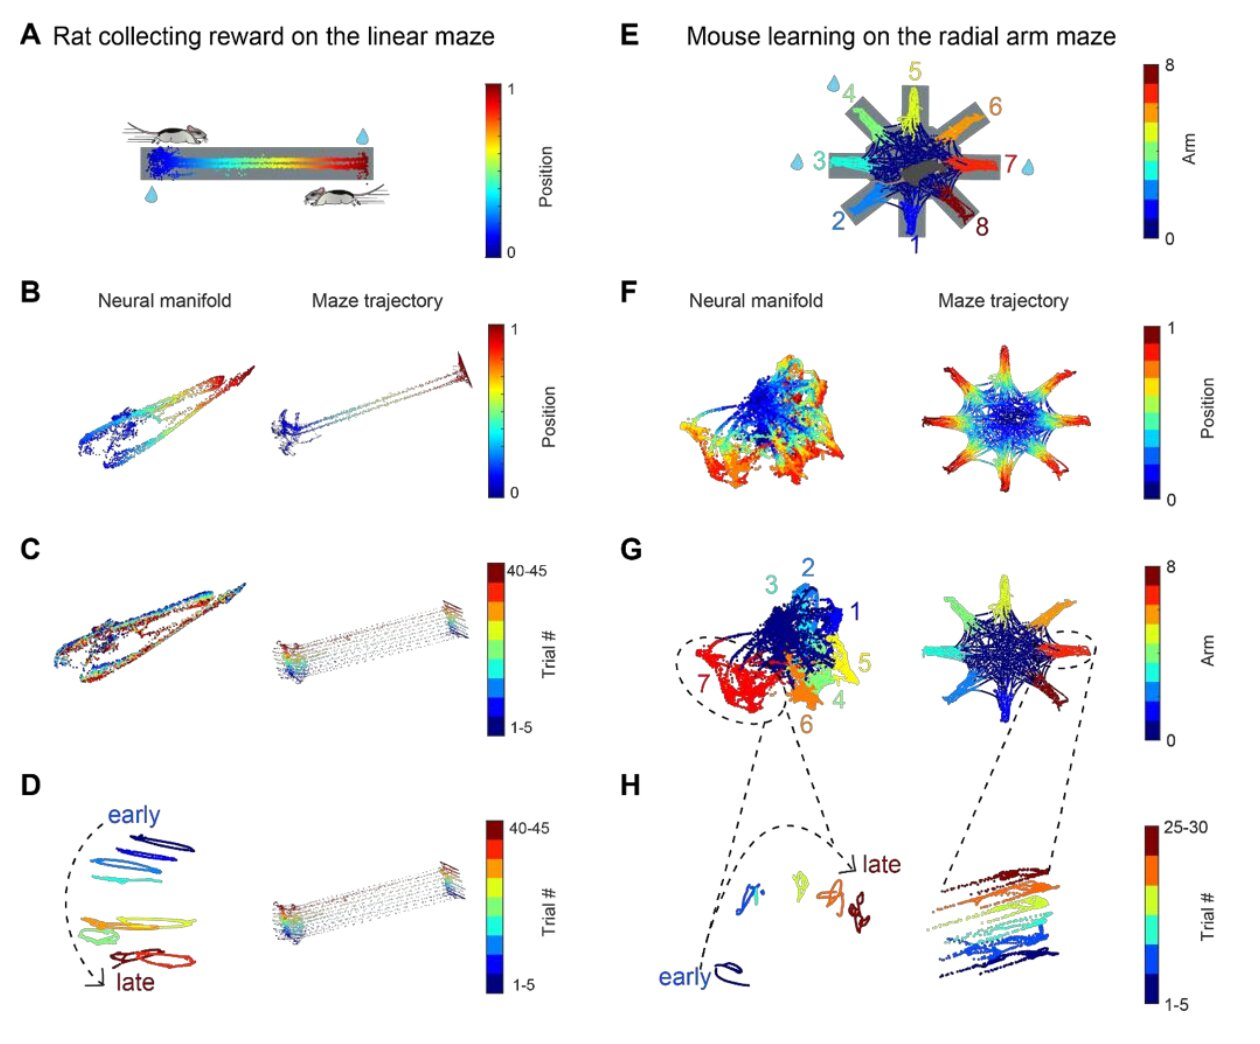
\includegraphics[width=\textwidth]{figures/ch_selection2024/Extended_Fig2.jpg}
\caption[Extended Data Fig.~2: Trial-specific evolution of neuronal population activity in different tasks and rodent species]{\textbf{Extended Data Fig.~2: Trial-specific evolution of neuronal population activity in different tasks and rodent species.}
Maze topology and trial-specific population representation in the manifold of figure-eight maze were also observed in simpler tasks like a linear maze, as well as more complex tasks like radial arm maze.
(A) Rat running back and forth between the two reward ports located at either end of the linear track to collect water reward (blue droplets).
(B) Animal's trajectory along the track was color-coded by animals' linearized position along the track. Only data when the animal's speed was larger than 1 cm/s was included. Left, UMAP embedding of population activity, colored by the rat's linearized position. Right, running trajectory of a rat on the linear maze.
(C) Same session as (B) but the manifold (left) and maze trajectory (right) were colored by trial block number.
(D) Same session as (B) and (C), but using semi-supervised UMAP trained on blocks of 5 trials. The neural manifold (left) and maze trajectory (right) were colored by trial block number.
(E) In the radial-arm maze experiment, mouse collect water reward from 3 out of the 8 potential reward sites at the end of each arm. The animal's trajectory along the track was color-coded by the arm's identity.
(F) Left, UMAP embedding of population activity, colored by animal's linearized position on each of the 8 arms. Right, running trajectory of a mouse on the radial arm maze.
(G) Same session as (F) but the neural manifold and maze trajectory were colored by arm identity.
(H) Neural manifold (left) was trained using semi-supervised UMAP on blocks of 5 trials. The manifold (left) and maze trajectory (right) were colored by trial block number.}
\label{fig:selection2024-ext2}
\end{figure}

\begin{figure}[htbp]
\centering
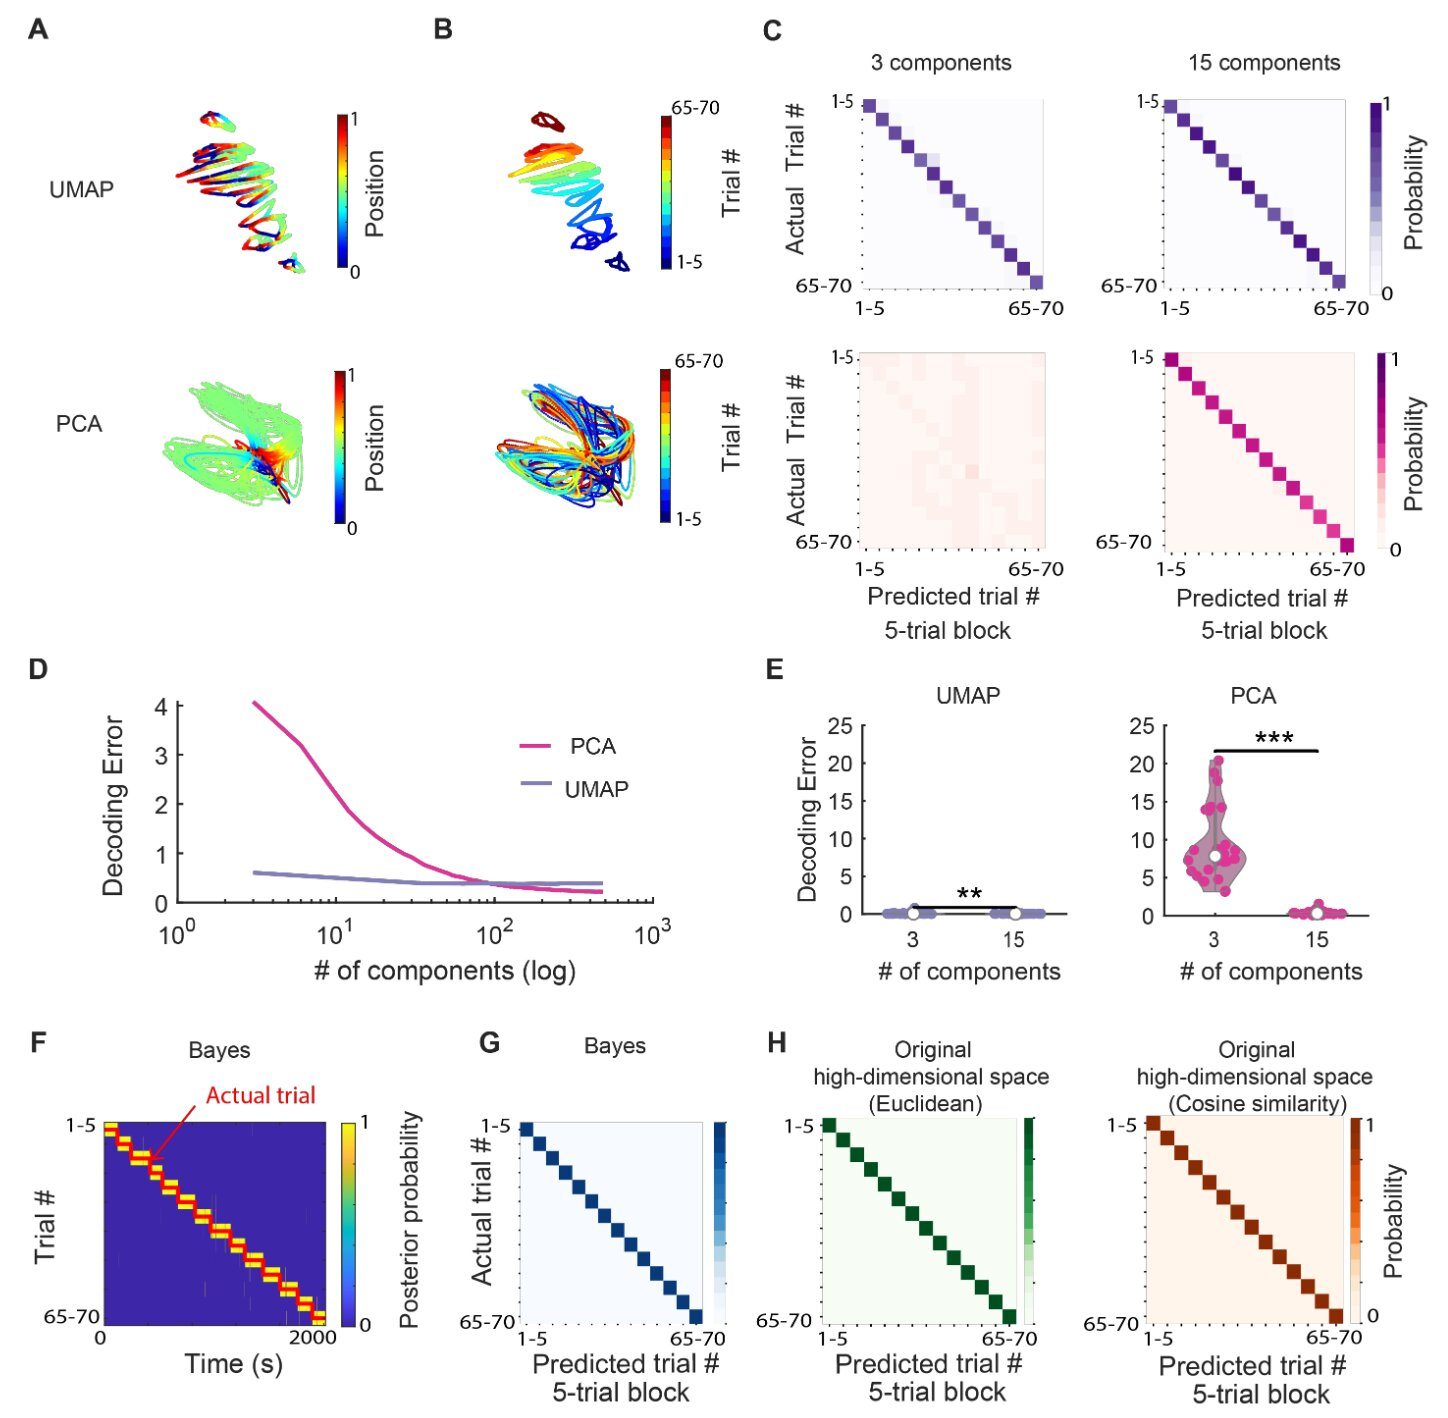
\includegraphics[width=\textwidth]{figures/ch_selection2024/Extended_Fig3.jpg}
\caption[Extended Data Fig.~3: Trial block identity can be decoded using five different methods]{\textbf{Extended Data Fig.~3: Trial block identity can be decoded using five different methods.}
(A) Low-dimensional embedding of CA1 population activity, colored by animal's linearized position on the figure-eight maze. Top, UMAP manifold. Bottom, PCA manifold.
(B) Same as (A) but colored by trial block number.
(C) Confusion matrix of trial block decoding result using 3 (left) and 15 (right) components of the low-dimensional data from an example session. Top, UMAP decoding results. Bottom, PCA decoding results.
(D) Decoding error as a function of the number of components in the low-dimensional space for both UMAP and PCA decoding.
(E) Summary statistics across the whole dataset, comparing decoding accuracy using UMAP and PCA using the first 3 and 15 principal components. PCA decoding achieved a similar level of decoding accuracy as UMAP when decoded based on the first 15 principal components (**$P < 0.01$ and ***$P < 10^{-9}$ for UMAP and PCA respectively; paired t-test; $n = 26$ sessions from 6 animals).
(F) Posterior probability of Bayesian trial block decoding across time in one session. Red line, actual trial block number.
(G) Confusion matrix of trial block decoding results from Bayesian decoding for the same example session shown in (C).
(H) Confusion matrix of trial block decoding results from the original high-dimensional space for the same example session shown in (C) and (G). Left, Euclidean distance was used as the distance metric. Right, cosine similarity was used as the distance metric.}
\label{fig:selection2024-ext3}
\end{figure}

\begin{figure}[htbp]
\centering
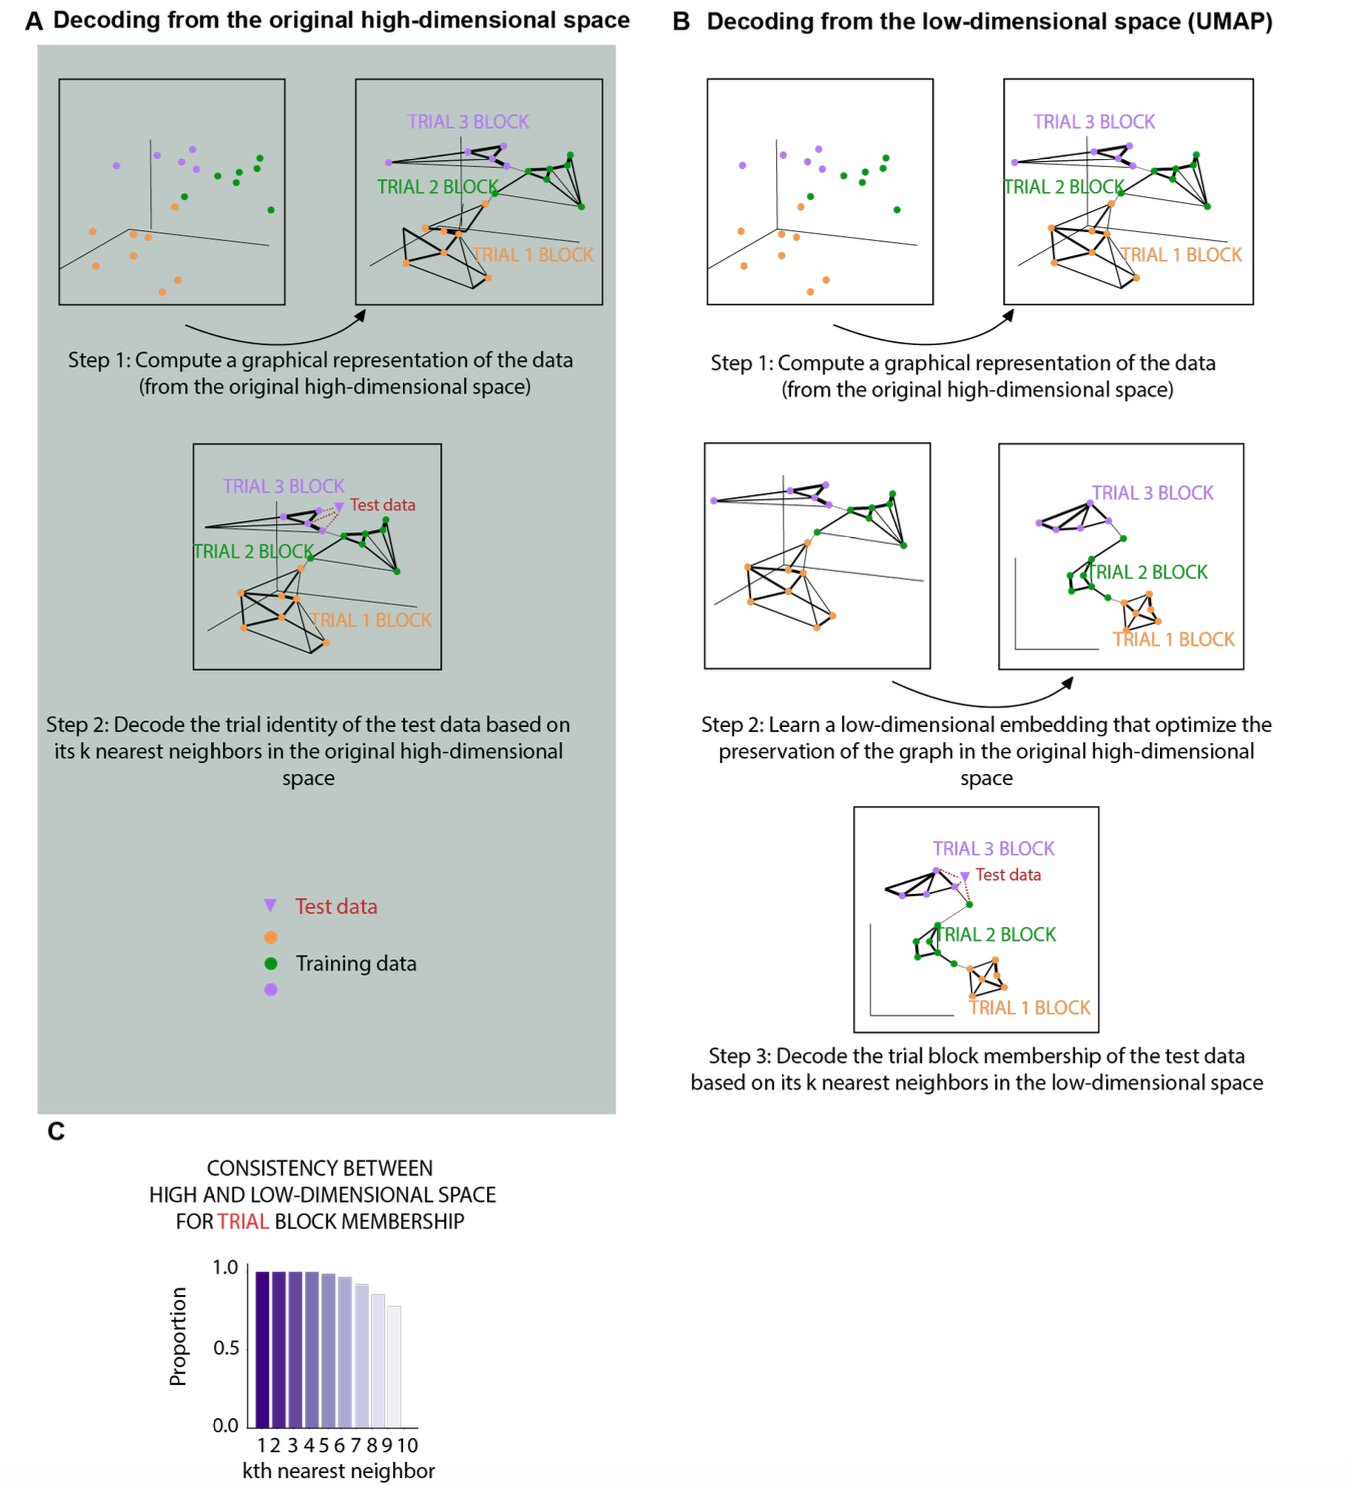
\includegraphics[width=\textwidth]{figures/ch_selection2024/Extended_Fig4.jpg}
\caption[Extended Data Fig.~4: Consistent trial block membership between the low-dimensional and the original high-dimensional space]{\textbf{Extended Data Fig.~4: Consistent trial block membership between the low-dimensional and the original high-dimensional space.}
(A) Diagram explaining the main steps of trial block decoding from the original high-dimensional space. Step 1: by default, a weighted kNN graph, which connects each datapoint to its k nearest neighbors, was constructed and used to generate the initial topological representation of the training dataset. Step 2: the trial block membership of the test data (purple triangle) was decoded by taking the mode of its k nearest neighbors.
(B) Diagram explaining the main steps of trial block decoding from the low-dimensional space generated by UMAP. Step 1 was the same as in (A). Step 2: optimize the low-dimensional representation to preserve the topological representation. Step 3: the trial block membership of the test data was decoded by taking the mode of its k nearest neighbors in the low-dimensional embedding.
(C) To check whether the UMAP dimensionality reduction process introduced distortions that affected the decoded trial block membership (5-trial block), the consistency between the original high-dimensional space and reduced low-dimensional space was plotted. For each data point, the decoded trial block membership of its ten nearest neighbors in the high-dimensional space and the reduced low-dimensional space were compared. A data point was considered as having consistent trial block membership if they were decoded to the same trial block. For the first four nearest neighbors, the decoded trial block membership between the high and low-dimensional space was 100\% consistent. Thus, UMAP dimensionality reduction did not introduce any distortion at the level of trial block decoding.}
\label{fig:selection2024-ext4}
\end{figure}

\begin{figure}[htbp]
\centering
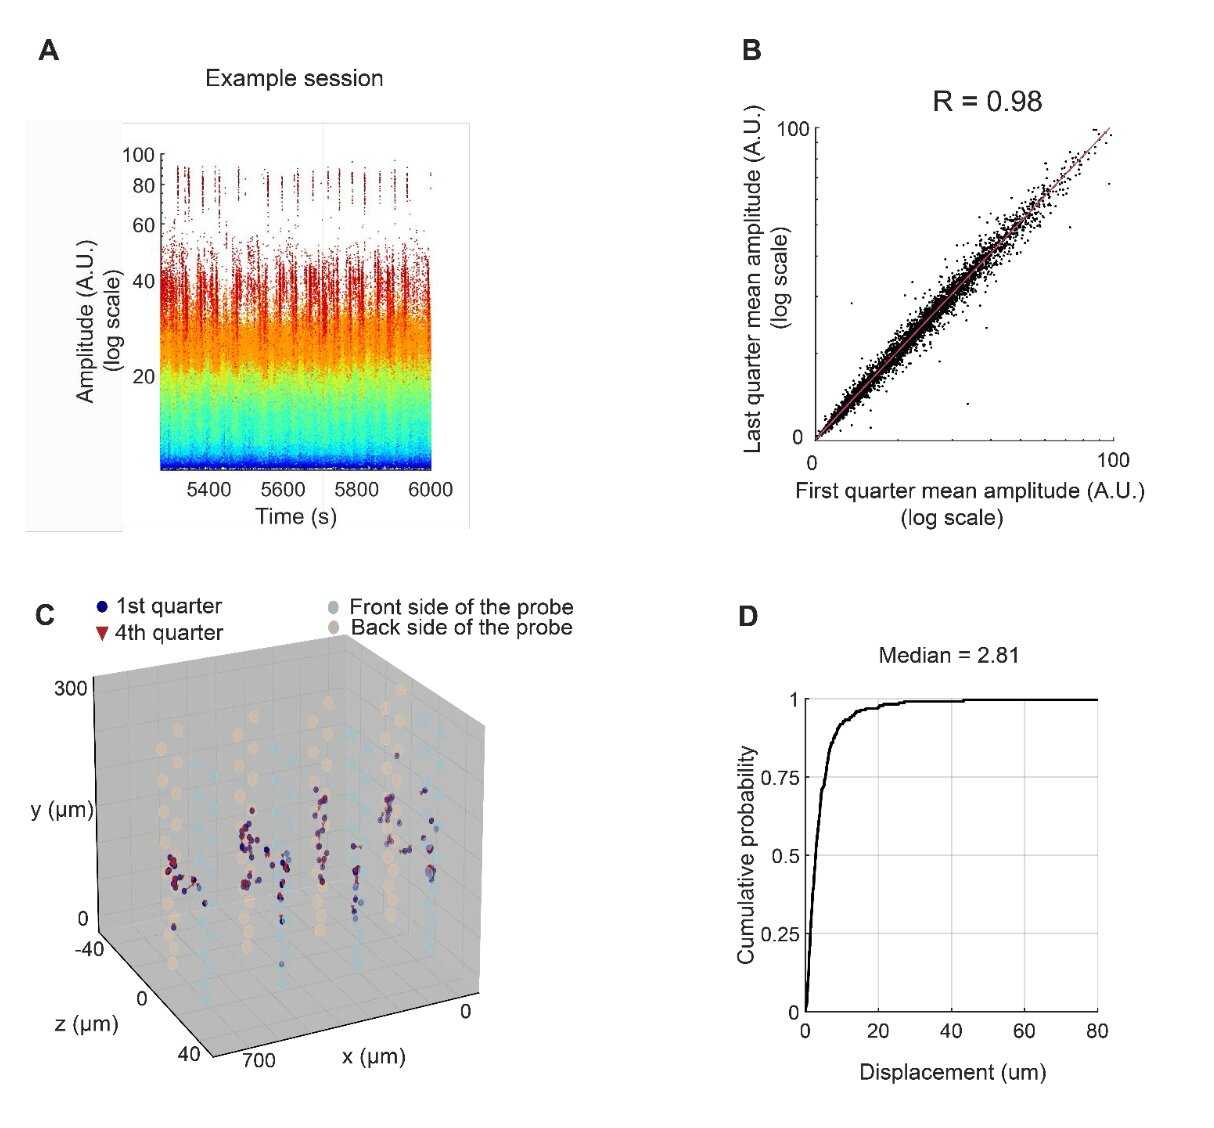
\includegraphics[width=\textwidth]{figures/ch_selection2024/Extended_Fig5.jpg}
\caption[Extended Data Fig.~5: Assessment of single-unit stability over time]{\textbf{Extended Data Fig.~5: Assessment of single-unit stability over time.}
(A) Waveform amplitude over time (on-maze duration) for all the cells in an example session. Spikes of individual neurons are color-coded by amplitude.
(B) Scatter plot of waveform amplitude in the first quarter of on-maze recording compared to the last quarter, for all the isolated units from the entire figure-eight maze dataset (Pearson correlation coefficient, $R = 0.98$, $P < 10^{-32}$; $N = 4469$ cells from 6 animals).
(C) Single-unit waveform centroid displacement across time, from a representative session, plotted in 3-D space. Centroid was computed by taking the spatial average across electrode positions weighted by the squared mean waveform amplitude at each electrode. Waveform centroid for each single unit during the first quarter (blue circles) and last quarter of recording (red triangles) were connected by red lines.
(D) Cumulative distribution of unit centroid displacement between the first and the last quarter of maze recording for all the cells in the dataset (median = 2.81-$\mu$m, Q1 = 1.37-$\mu$m, Q3 = 5.46-$\mu$m; $N = 4469$ cells from 6 animals).}
\label{fig:selection2024-ext5}
\end{figure}

\begin{figure}[htbp]
\centering
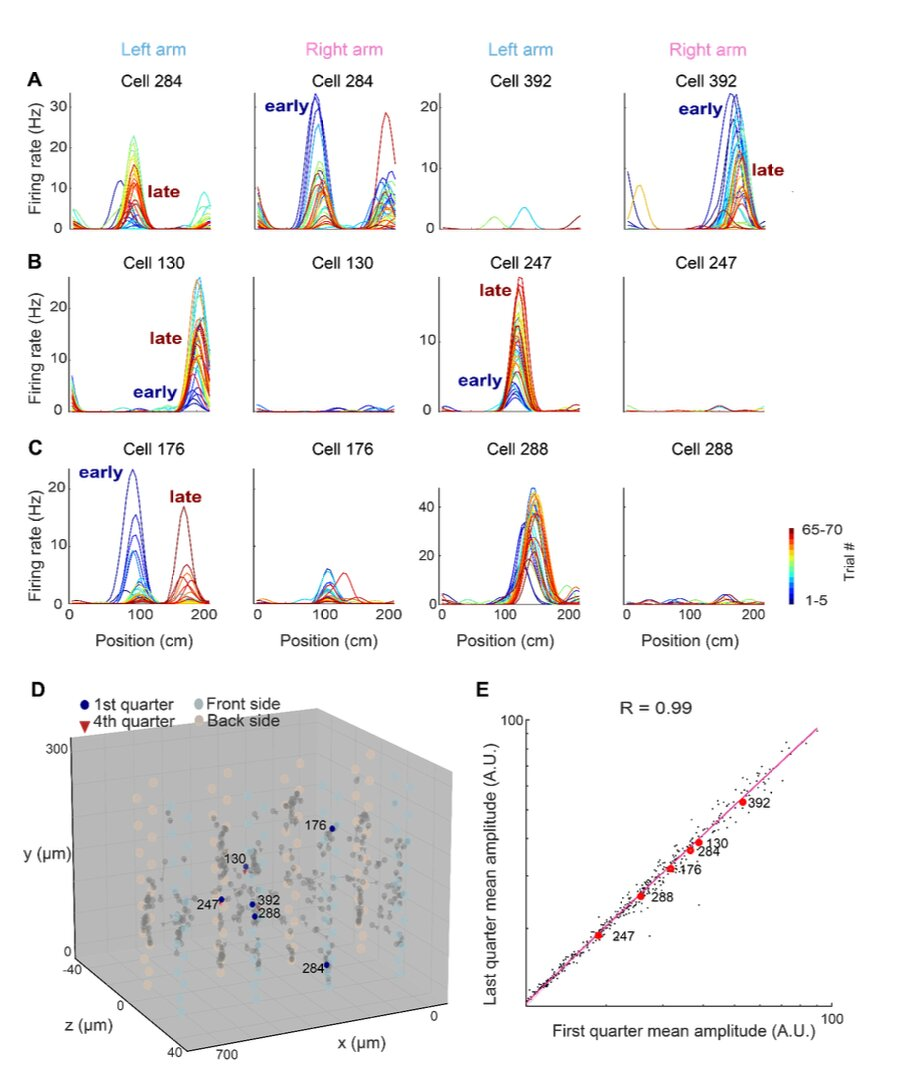
\includegraphics[width=\textwidth]{figures/ch_selection2024/Extended_Fig6.jpg}
\caption[Extended Data Fig.~6: Spatial tuning curve across trials of example neurons]{\textbf{Extended Data Fig.~6: Spatial tuning curve across trials of example neurons.}
The firing rate in space (linearized position on the figure-eight maze) of 6 example neurons across different trials in one representative session. The tuning curves were color-coded by trial block number (cold color for early trials and warm color for late trials). For each example cell, its firing rates as a function of the linearized position (from 0 to 200-cm) for each of the two arms of the figure-eight maze were plotted separately.
(A) Two example cells that fired with higher firing rates during early trials. Left, left arm trials. Right, right arm trials.
(B) Two example cells that fired with higher firing rate during late trials.
(C) Two example cells with place field remapping across trials.
(D) Single unit waveform centroid displacement across time, plotted in 3D space, highlighting the 6 example cells shown in (A)--(C). Notice that the firing rates or place fields of all 6 example neurons varied across different trials but their location with respect to the electrode sites remained relatively stable.
(E) Scatter plot for waveform amplitude during the first versus the last quarter of recording, highlighting the 6 example cells (red dots) shown in (A)--(C) (Pearson correlation coefficient, $R = 0.99$, $P < 10^{-32}$).}
\label{fig:selection2024-ext6}
\end{figure}

\begin{figure}[htbp]
\centering
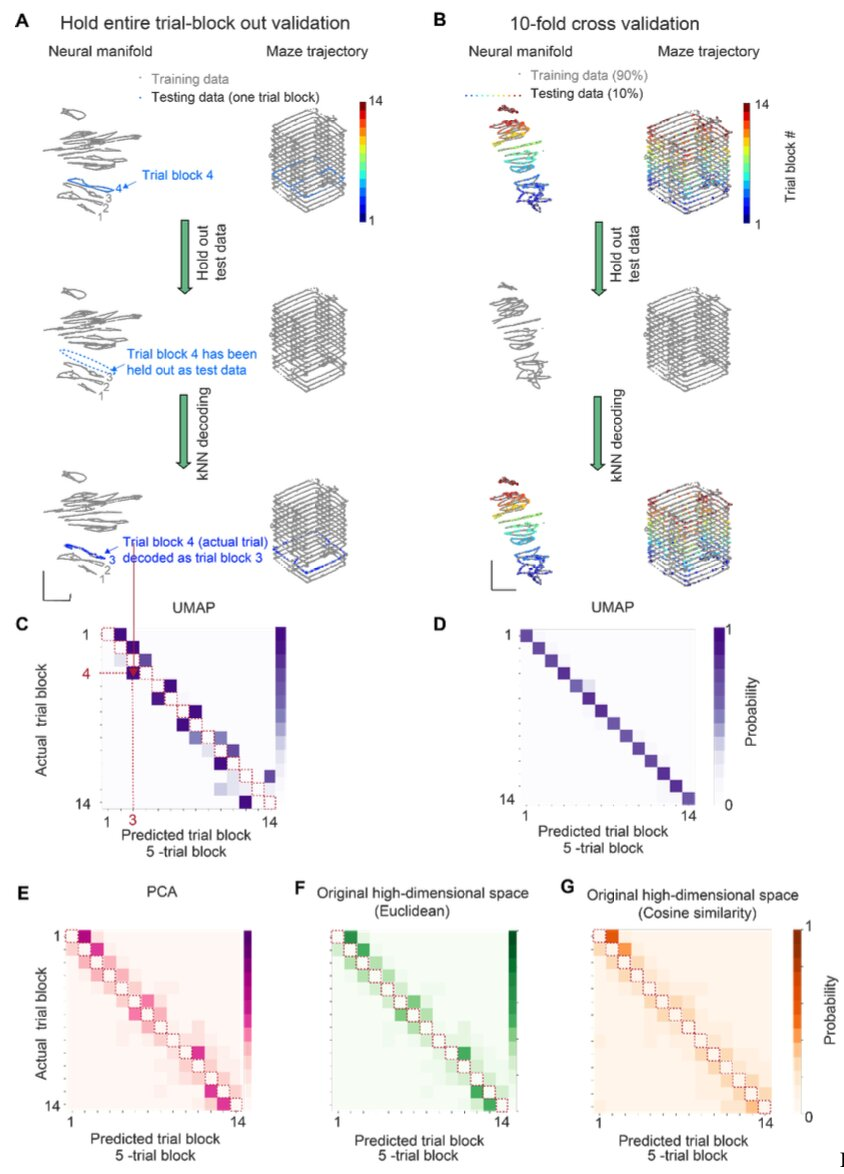
\includegraphics[width=\textwidth]{figures/ch_selection2024/Extended_Fig7.jpg}
\caption[Extended Data Fig.~7: Hold entire-trial-block-out validation results from four different decoding methods]{\textbf{Extended Data Fig.~7: Hold entire-trial-block-out validation results from four different decoding methods.}
(A) Illustration of the hold entire-trial-block-out validation method. Top, neural manifold from all the data in one example session. To give an example of the cross-validation procedure, data from one trial block (trial block 4; blue) was highlighted. Middle, the highlighted trial block was held out as test data. After removing the test data, a kNN decoder was trained only using training data (grey). Bottom, the test data was then embedded with the learned manifold and the kNN decoder was used for trial block membership decoding.
(B) Illustration of the 10-fold cross-validation method. Top, neural manifold generated from all the data in one example session. 10\% of the data were highlighted (colored by their true trial block identity). Middle, after removing the test data, a kNN decoder was trained only using training data (grey). Bottom, embedding the test data with the training manifold and using the kNN decoder for trial block identity decoding.
(C) Confusion matrix obtained using hold entire-trial-block-out validation. Note that the diagonal of the confusion matrix had 0 decoding probability because the training and test data did not share any data from the same trial block.
(D) Confusion matrix from UMAP trial block decoding using hold-entire-trial-block-out validation.
(E) Confusion matrix from UMAP trial block decoding using 10-fold cross-validation.
(F) Confusion matrix for trial block decoding from the original high-dimensional space, with Euclidean distance as the distance metric.
(G) Similar to (F), but using the cosine similarity as the distance metric.}
\label{fig:selection2024-ext7}
\end{figure}

\begin{figure}[htbp]
\centering
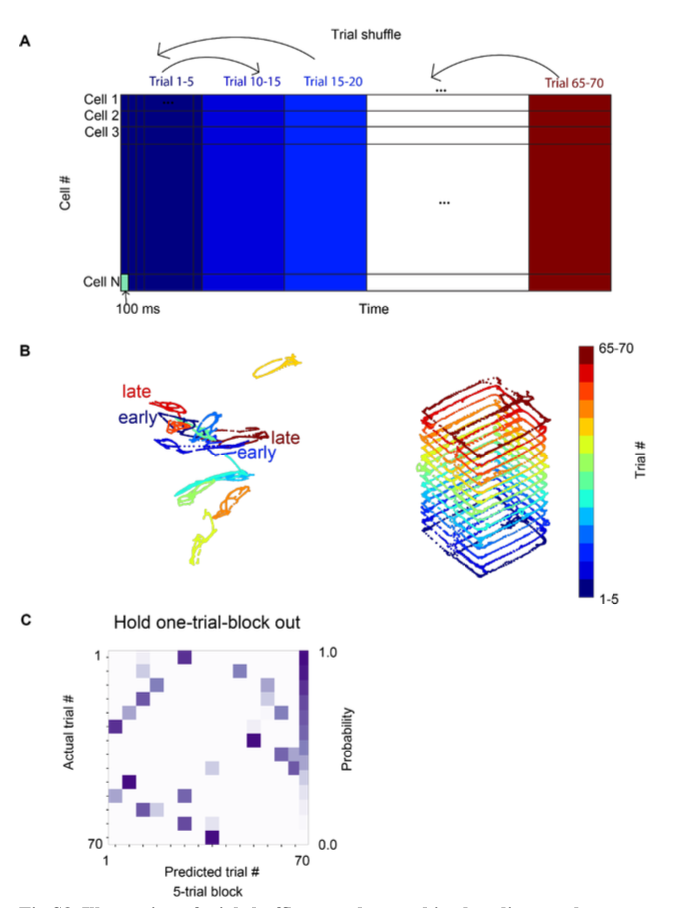
\includegraphics[width=\textwidth]{figures/ch_selection2024/Extended_Fig8.png}
\caption[Extended Data Fig.~8: Illustration of trial shuffle procedure and its decoding results]{\textbf{Extended Data Fig.~8: Illustration of trial shuffle procedure and its decoding results.}
(A) Illustration of the trial shuffle procedure. Neural spiking data was binned by 100-ms bins and concatenated into a matrix (each row is a cell, and each column is a 100-ms bin). Trial shuffle was performed by shuffling the trial block identity of the entire data matrix.
(B) Left, neural manifold for the trial-shuffled data. Both the neural manifold (left) and the maze trajectory (right) were colored by the trial block number. Notice that the shuffle procedure disrupted the structure of the data such that early and late trials may be embedded very close to each other.
(C) Confusion matrix of the trial shuffled data for hold-entire-trial-out validation. Trial shuffled data lost the trial structure in real data.}
\label{fig:selection2024-ext8}
\end{figure}

\begin{figure}[htbp]
\centering
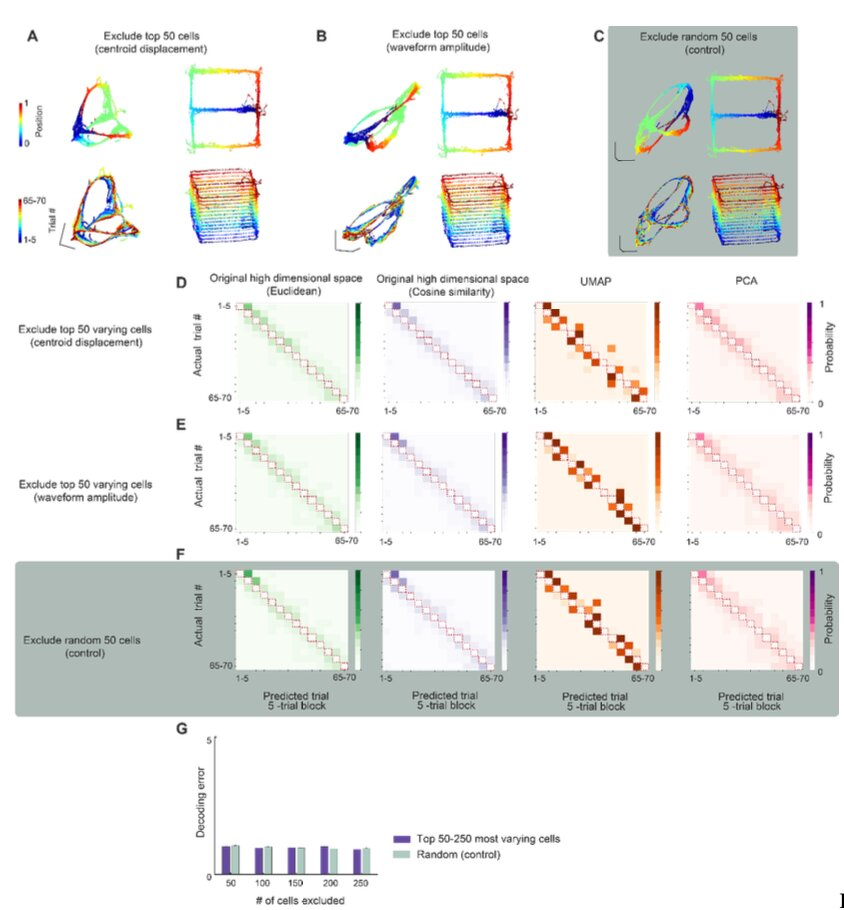
\includegraphics[width=\textwidth]{figures/ch_selection2024/Extended_Fig9.jpg}
\caption[Extended Data Fig.~9: Trial-by-trial representation drift cannot be explained by variations in waveform amplitude or waveform centroid displacement]{\textbf{Extended Data Fig.~9: Trial-by-trial representation drift cannot be explained by variations in waveform amplitude or waveform centroid displacement.}
The purpose of this figure was to test whether the trial-by-trial variation at the population level can be explained by electrode drift. Two metrics were measured: (1) waveform amplitude change and (2) waveform centroid displacement. Units were then sorted by those two metrics. Next, the top k cells with greatest variance for each of the metric were excluded from decoding analysis.
(A) The low-dimensional embedding after excluding 50 cells that showed the largest centroid displacement was plotted. The manifold was colored by animal's linearized position (top) and trial number (bottom).
(B) The low-dimensional embedding after excluding 50 cells with the greatest amplitude variance over time was plotted.
(C) The low-dimensional embedding after randomly excluding 50 cells (control) was plotted.
(D) Confusion matrices of trial block decoding results after excluding 50 cells with the largest centroid displacement. From left to right, decoding results from the original high-dimensional space using Euclidean distance (green), decoding from original high-dimensional space using cosine similarity (purple), UMAP decoding (orange), and PCA decoding (pink).
(E) Confusion matrices of trial block decoding results after excluding 50 cells that showed the largest amplitude variance.
(F) Confusion matrices of trial block decoding results after randomly removing 50 cells (control).
(G) Decoding error after excluding the top k most variant cells versus k random cells, where k ranged from 50--250 cells. The decoding error was not significantly different from control across different range of k.}
\label{fig:selection2024-ext9}
\end{figure}

\begin{figure}[htbp]
\centering
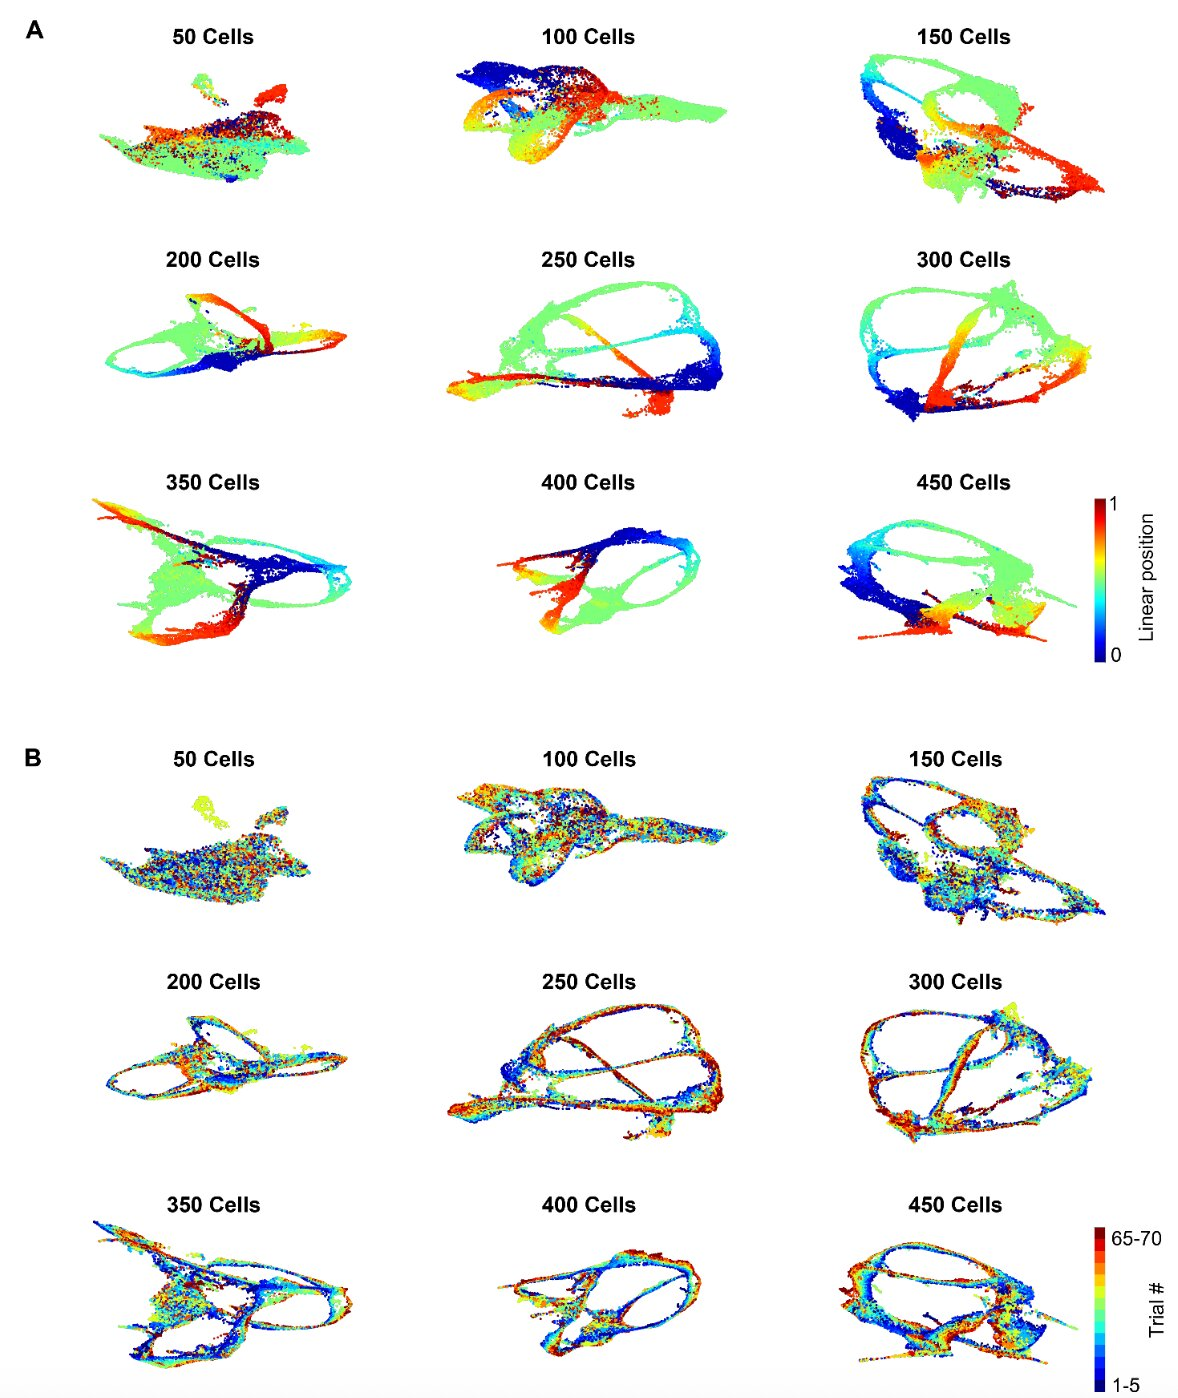
\includegraphics[width=\textwidth]{figures/ch_selection2024/Extended_Fig10.jpg}
\caption[Extended Data Fig.~10: Visualization of the downsampling analysis using UMAP (unsupervised)]{\textbf{Extended Data Fig.~10: Visualization of the downsampling analysis using UMAP (unsupervised).}
(A) Manifolds generated from downsampling the number of cells included for UMAP embedding. Manifolds were colored by the animal's linearized position.
(B) Same as in (A) but manifolds were colored by trial block number.}
\label{fig:selection2024-ext10}
\end{figure}

\begin{figure}[htbp]
\centering
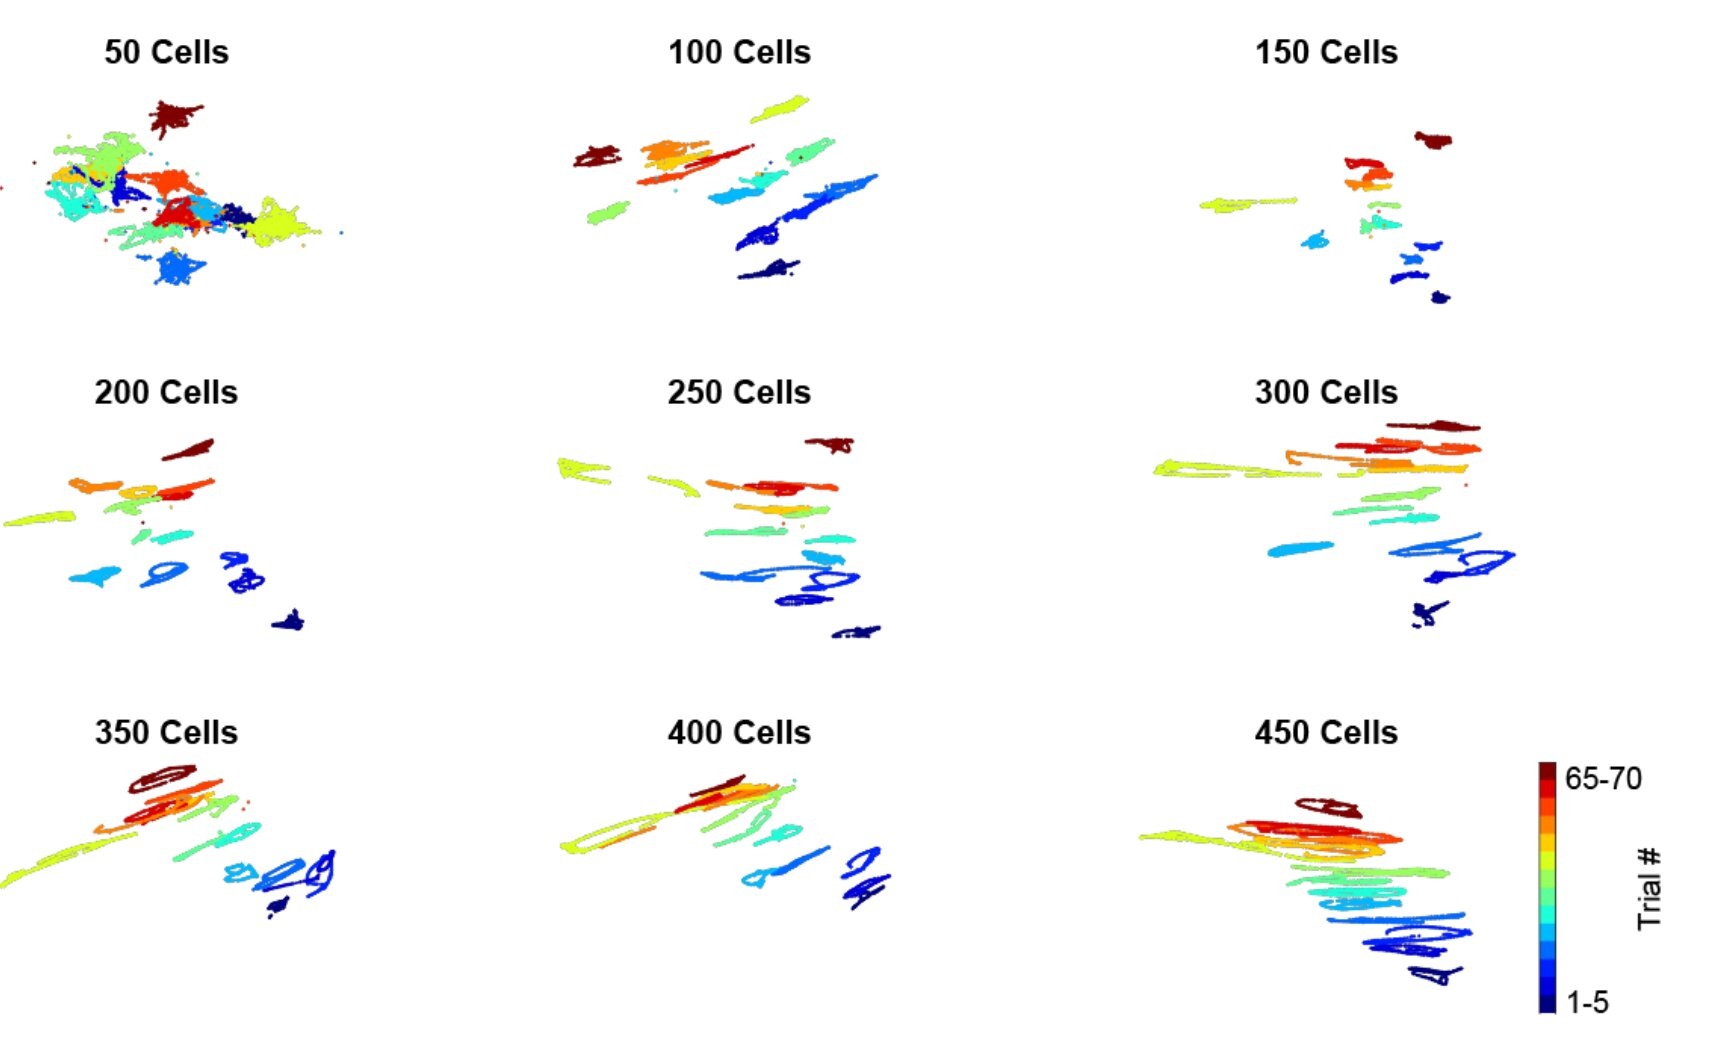
\includegraphics[width=\textwidth]{figures/ch_selection2024/Extended_Fig11.jpg}
\caption[Extended Data Fig.~11: Visualization of downsampling analysis UMAP (semi-supervised)]{\textbf{Extended Data Fig.~11: Visualization of downsampling analysis UMAP (semi-supervised).}
UMAP manifolds generated from downsampling the number of cells. Here, the manifold embeddings were trained by the semi-supervised method. Manifolds were colored by trial block number.}
\label{fig:selection2024-ext11}
\end{figure}

\begin{figure}[htbp]
\centering
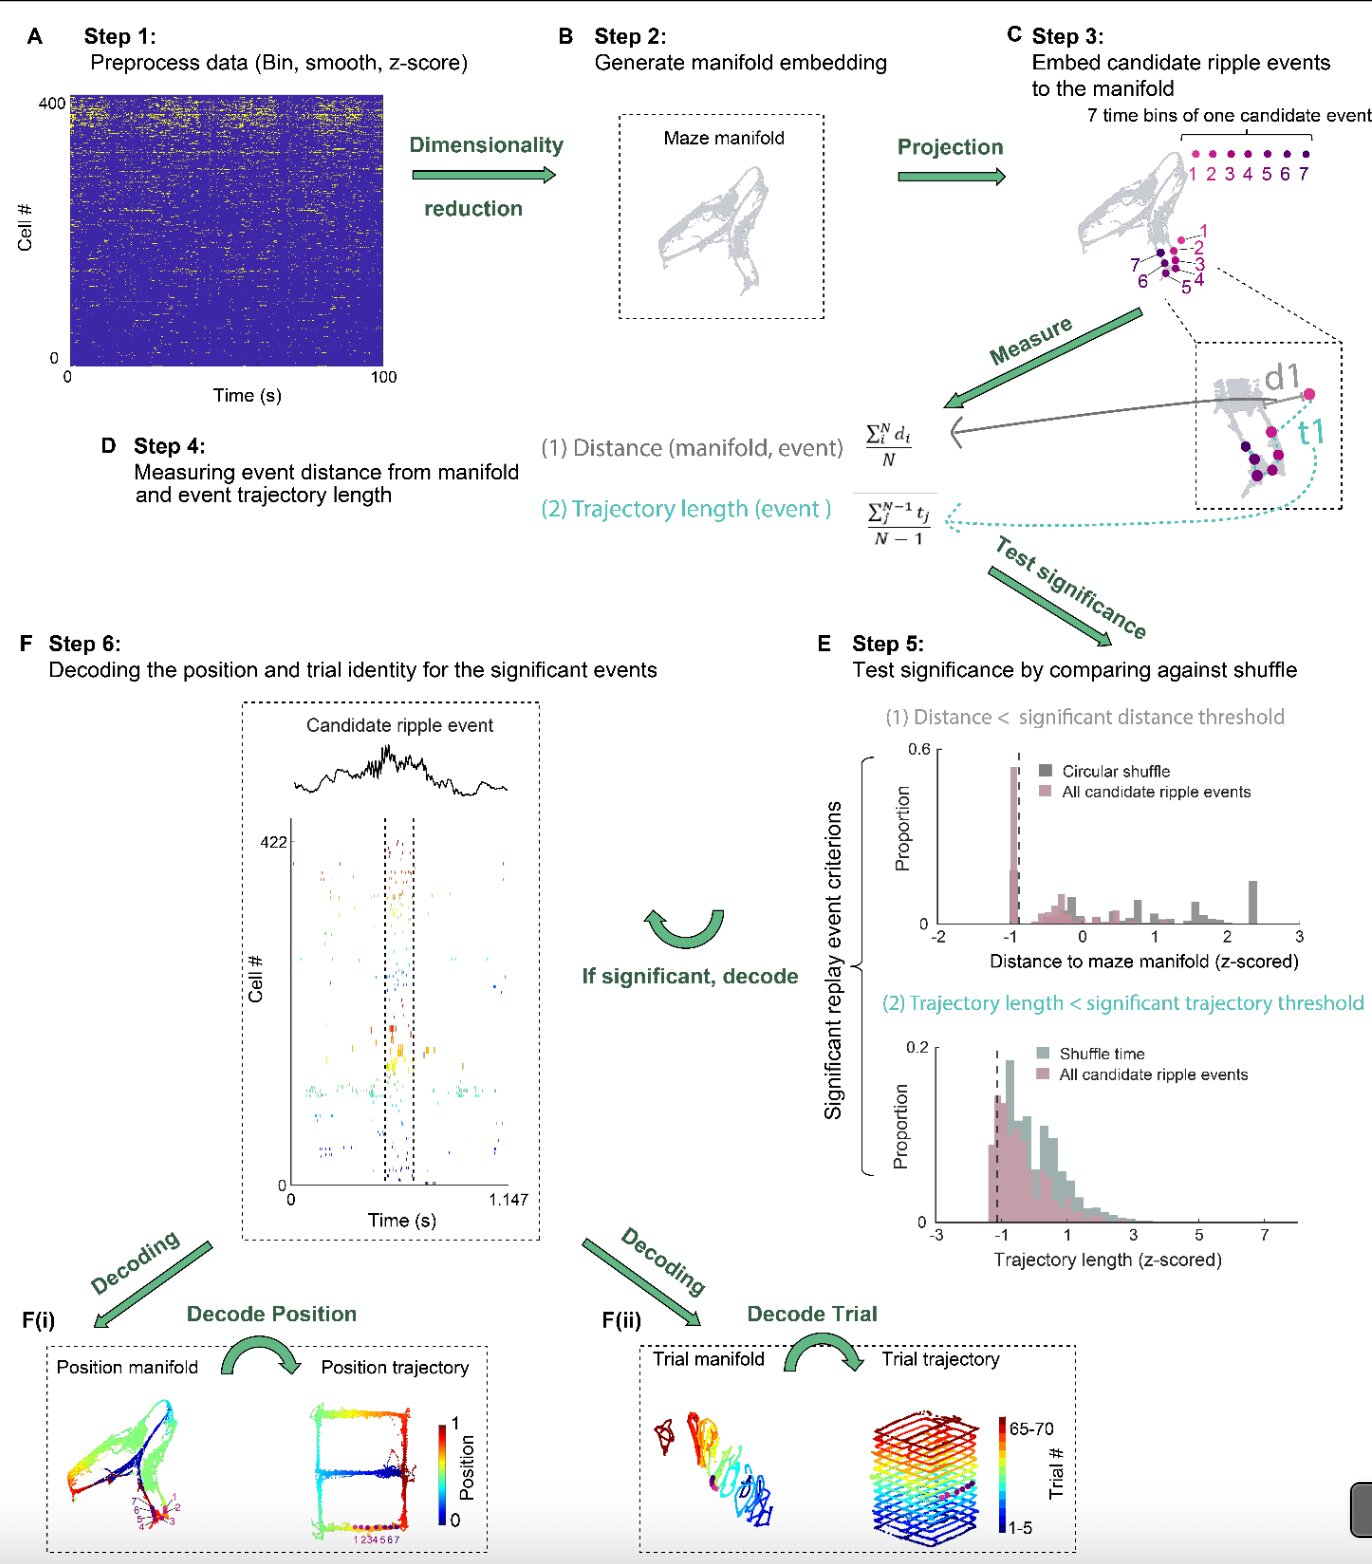
\includegraphics[width=\textwidth]{figures/ch_selection2024/Extended_Fig12.jpg}
\caption[Extended Data Fig.~12: Flow diagram demonstrating procedures for detecting and decoding significant SPW-R replays]{\textbf{Extended Data Fig.~12: Flow diagram demonstrating procedures for detecting and decoding significant SPW-R replays.}
(A) Step 1: Preprocessing. The animal performed an alternation task in the figure-eight maze while spikes from 422 pyramidal cells were recorded. Spike trains during maze learning were binned in 100-ms bins, z-scored, and then smoothed. Spike trains of candidate SPW-R events were binned into 20-ms bins, smoothed, and then z-scored.
(B) Step 2: Generating maze manifold embedding. The preprocessed data matrix was passed through dimensionality reduction step by either UMAP or PCA, which generated a low-dimensional embedding.
(C) Step 3: Embedding candidate ripple events to the embedding metric defined by the maze manifold. The 7 pink-purple dots on the manifold represent low-dimensional embeddings of an example candidate SPW-R event.
(D) Step 4: Measuring distance to the manifold and trajectory length. The event distance to the manifold is defined as the mean Euclidean distance across all time bins within the event. The event trajectory length was defined as the mean trajectory length between all successive time bins.
(E) Step 5: Testing whether the candidate events were significant against shuffled distributions. A candidate event was classified as a significant replay event only if it satisfied two criteria.
(F) Step 6: Only significant replays were included for further analysis. F(i). To decode the virtual position relayed by the candidate event, the population activity during SPW-R was embedded with the position manifold. F(ii). Similarly, the SPW-R activity vectors were embedded with the trial manifold for trial block identity decoding.}
\label{fig:selection2024-ext12}
\end{figure}

\begin{figure}[htbp]
\centering
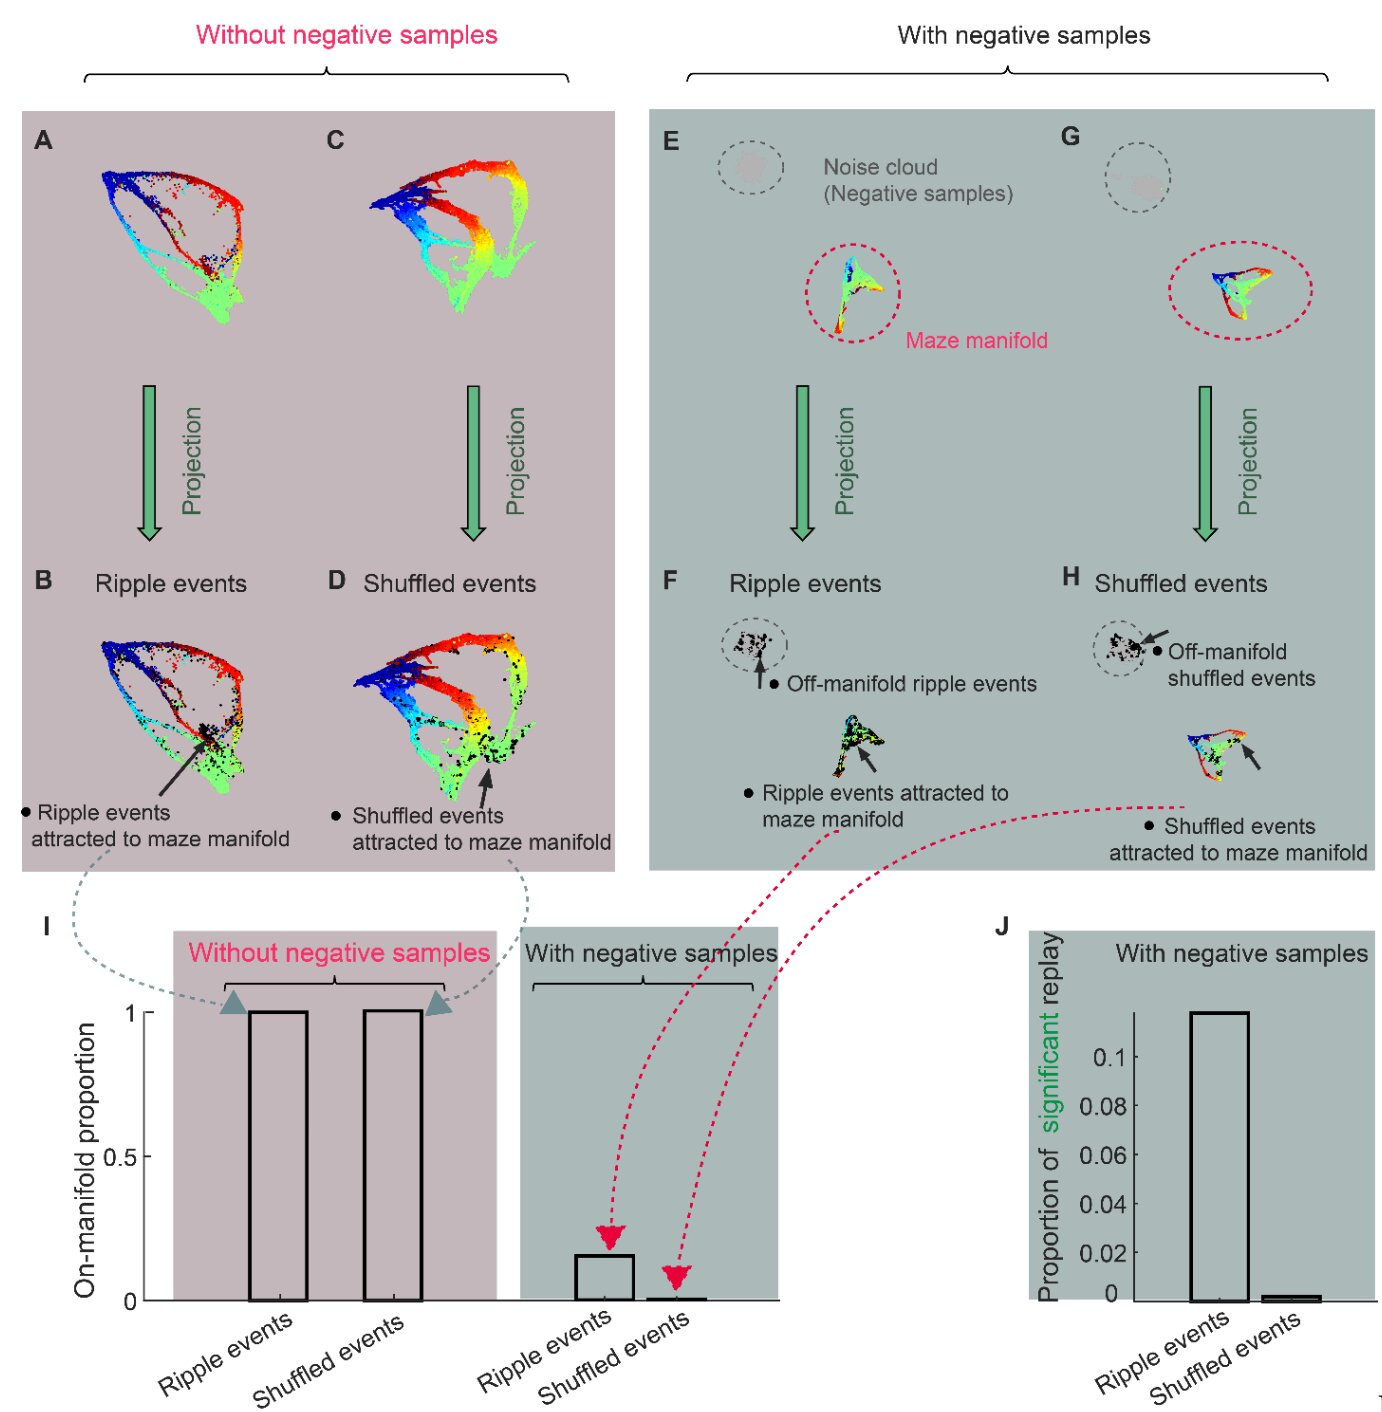
\includegraphics[width=\textwidth]{figures/ch_selection2024/Extended_Fig13.jpg}
\caption[Extended Data Fig.~13: Negative sampling algorithm and the role of negative samples]{\textbf{Extended Data Fig.~13: Negative sampling algorithm and the role of negative samples.}
(A) Generating UMAP embedding from maze data.
(B) Population vectors during SPW-R events were embedded with the maze manifold. Note that without negative samples, almost all SPW-R events were forced to be attracted to the maze manifold.
(C) and (D) were similar to (A) and (B), but embedded with shuffled SPW-R events.
(E) To avoid mode collapse, negative samples (grey dots) were generated and embedded along with the maze manifold so that data that were not similar to the maze data were attracted to the negative sample cloud. Negative samples were generated by shuffling the maze data.
(F) With the presence of negative samples, only SPW-R events (black) that were sufficiently similar to the maze manifold replay were attracted to the maze manifold.
(G) and (H) are similar to (E) and (F), but for the shuffled SPW-R events.
(I) Proportion of on-manifold events under different conditions. Without negative samples, all SPW-R events and shuffled data were equally close to the manifold. In contrast, with negative samples, only 15\% of real SPW-R events and 0.2\% of shuffled events were on-manifold.
(J) For an event to be classified as a significant replay event, it needs to be: (1) closer to the maze manifold compared to shuffle, (2) have a shorter trajectory length compared to shuffle. Approximately 11\% of the SPW-R events were significant replay events, whereas only 0.1\% of the shuffle events satisfy both significance criteria.}
\label{fig:selection2024-ext13}
\end{figure}

\begin{figure}[htbp]
\centering
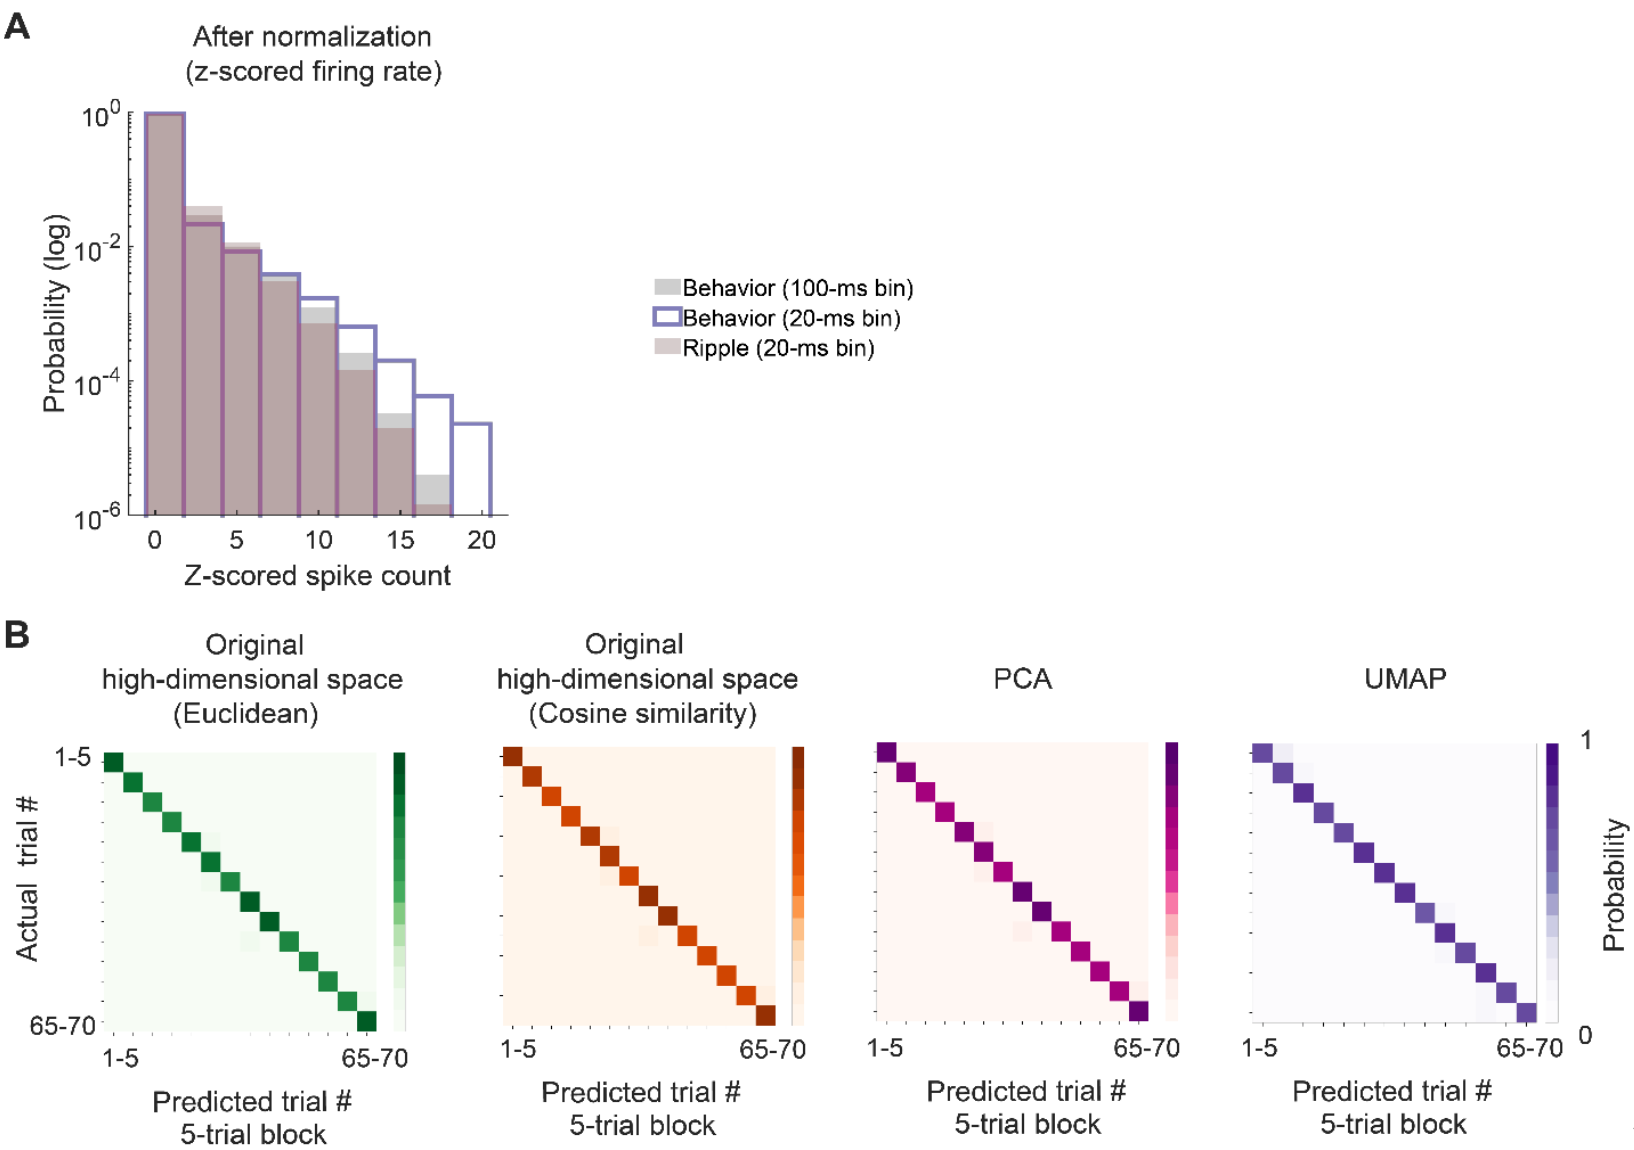
\includegraphics[width=\textwidth]{figures/ch_selection2024/Extended_Fig14.png}
\caption[Extended Data Fig.~14: Difference in time bin and its consequences for decoding]{\textbf{Extended Data Fig.~14: Difference in time bin and its consequences for decoding.}
(A) Distribution of spike counts with different time bins after normalization. As a standard preprocessing procedure, data were first z-scored before going through any dimensionality reduction analysis. After z-scoring, the distribution of spike counts was not different during maze behavior and SPW-Rs.
(B) To examine if difference in time bin affect the decoding result, test data with 20-ms bin were decoded from training data binned in 100-ms bins. Confusion matrix of decoding results obtained by embedding the data with 20-ms bins with the manifold generated by maze data with 100-ms bins. The decoding probability was concentrated at the diagonal of the confusion matrix, suggesting that trial block membership can still be accurately decoded, even with different time bins.}
\label{fig:selection2024-ext14}
\end{figure}

\begin{figure}[htbp]
\centering
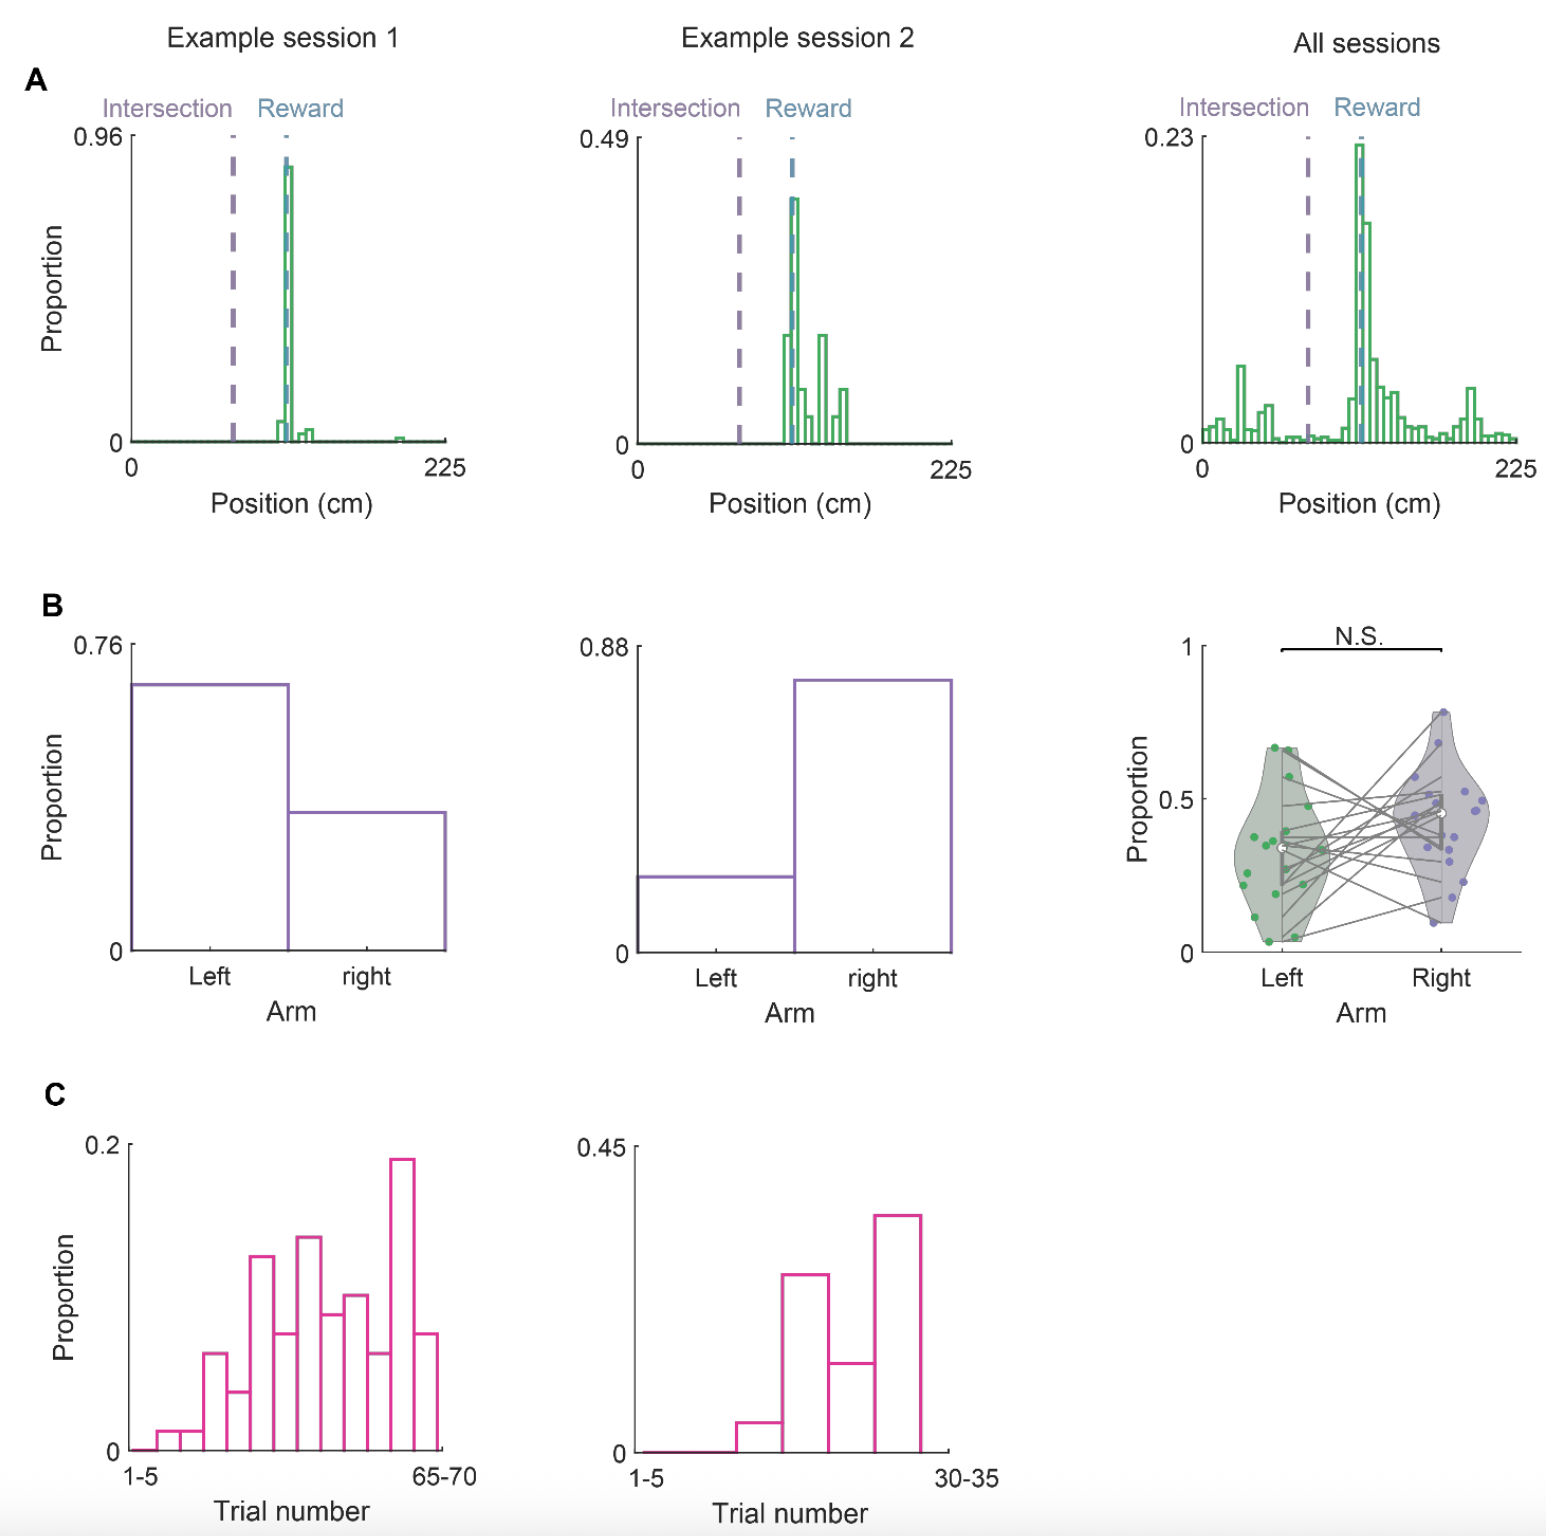
\includegraphics[width=\textwidth]{figures/ch_selection2024/Extended_Fig15.png}
\caption[Extended Data Fig.~15: Distribution of SPW-Rs across different locations, trials, and arms of the maze]{\textbf{Extended Data Fig.~15: Distribution of SPW-Rs across different locations, trials, and arms of the maze.}
(A) Distributions of SPW-Rs across different maze locations of the figure-eight maze from two example sessions and the summary data across all figure-eight maze sessions ($n = 21$ sessions from 6 animals). Intersection (purple dashed line), T junction of the figure-eight maze. Reward (blue dashed line), location of the water reward. Most of the awake replay events occur at the reward site.
(B) Distributions of SPW-Rs across different sides of the arms of the figure-eight maze from two example sessions and the summary data across all figure-eight maze sessions (N.S., not significant; unpaired t-test; $n = 21$ sessions from 6 animals).
(C) Distributions of SPW-Rs across different trial blocks of the figure-eight maze from two example sessions.}
\label{fig:selection2024-ext15}
\end{figure}

\begin{figure}[htbp]
\centering
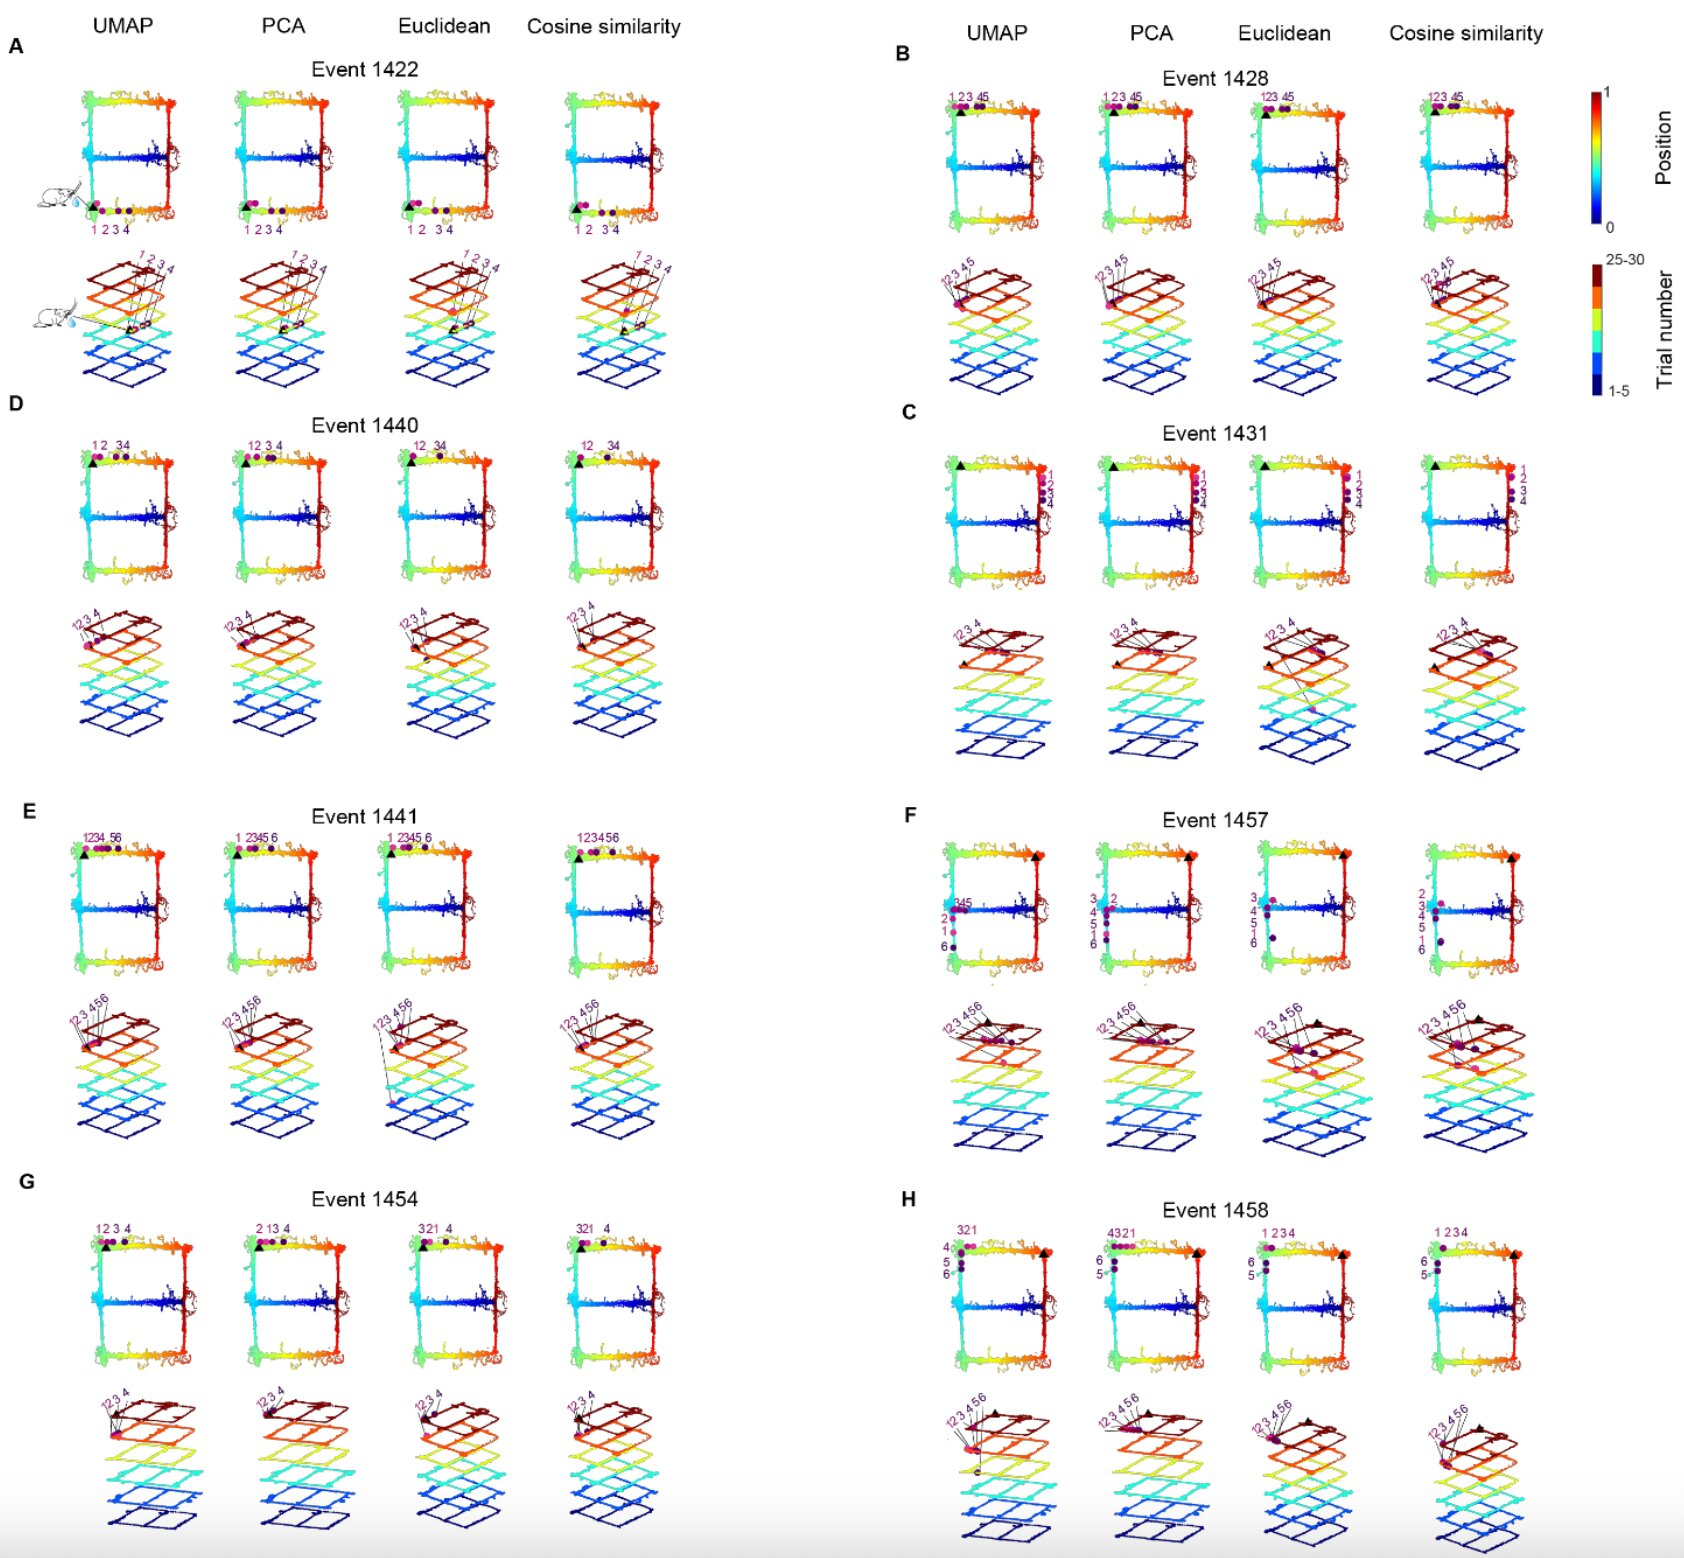
\includegraphics[width=\textwidth]{figures/ch_selection2024/Extended_Fig16.jpg}
\caption[Extended Data Fig.~16: Decoding results of example replay events using different decoding methods]{\textbf{Extended Data Fig.~16: Decoding results of example replay events using different decoding methods.}
(A)--(H) Example replay events from an example session. For each event, the top rows are position decoding results and the bottom rows are trial block decoding results. For each event, there are four columns of results each obtained from a different decoding method.}
\label{fig:selection2024-ext16}
\end{figure}

\begin{figure}[htbp]
\centering
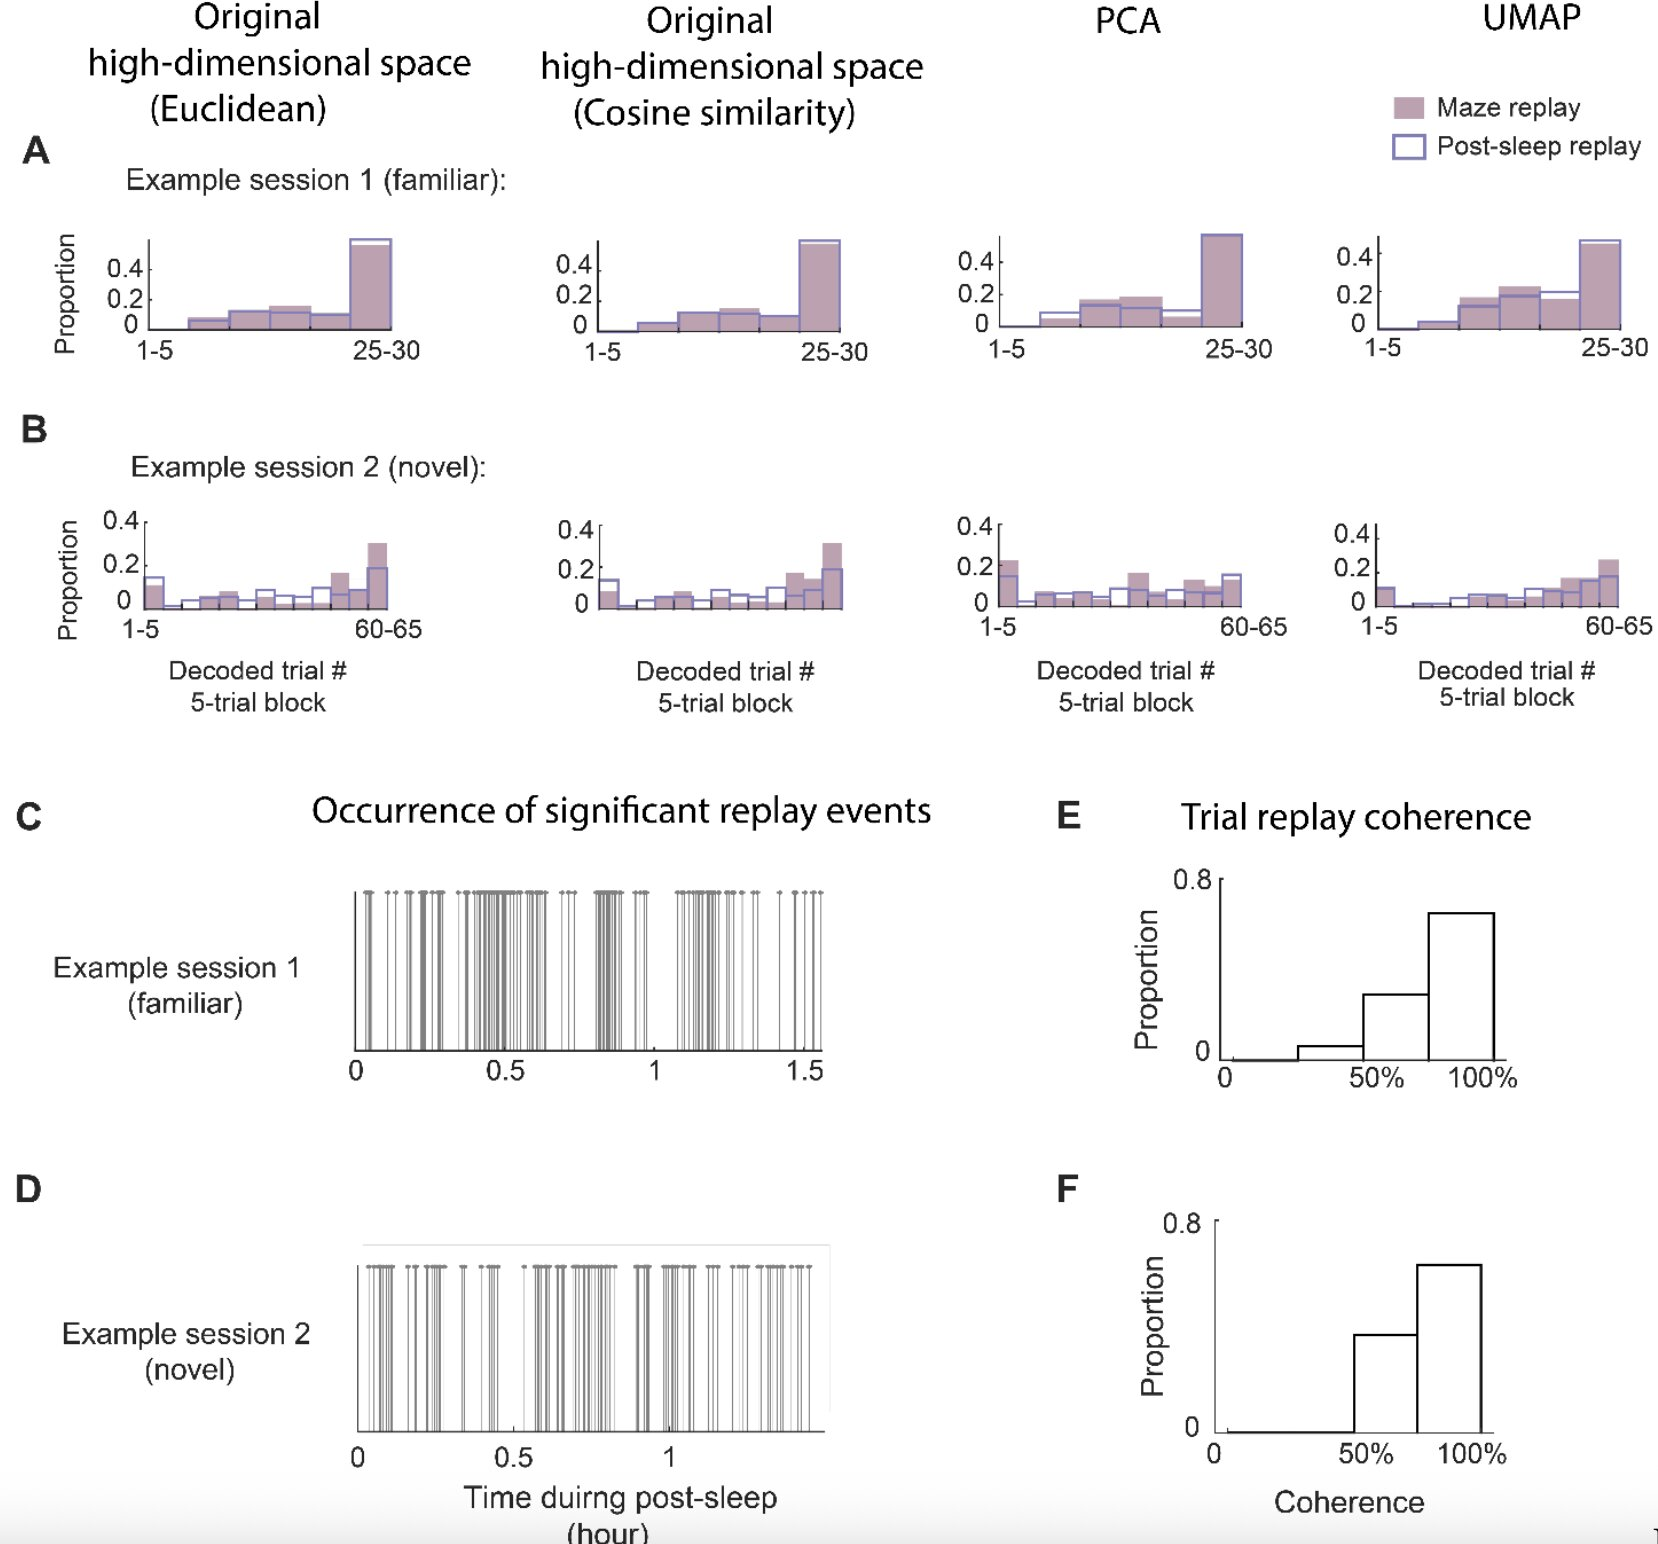
\includegraphics[width=\textwidth]{figures/ch_selection2024/Extended_Fig17.jpg}
\caption[Extended Data Fig.~17: Significant replay events and their decoding results in two example sessions]{\textbf{Extended Data Fig.~17: Significant replay events and their decoding results in two example sessions.}
(A)--(B) Trial distribution pattern for awake replay and post-sleep replay for two example sessions using 4 different decoding methods.
(C)--(D) Distribution of significant replay events over the course of post-sleep session (each grey line indicates the occurrence of one significant replay event).
(E)--(F) Distribution of within-event replay coherence for significant replay events. The coherency of each event was measured as the proportion of time bins that shared the same trial block label as the mode for that event. 100\% means all time bins of a given replay event were decoded to the same trial block label.}
\label{fig:selection2024-ext17}
\end{figure}

\begin{figure}[htbp]
\centering
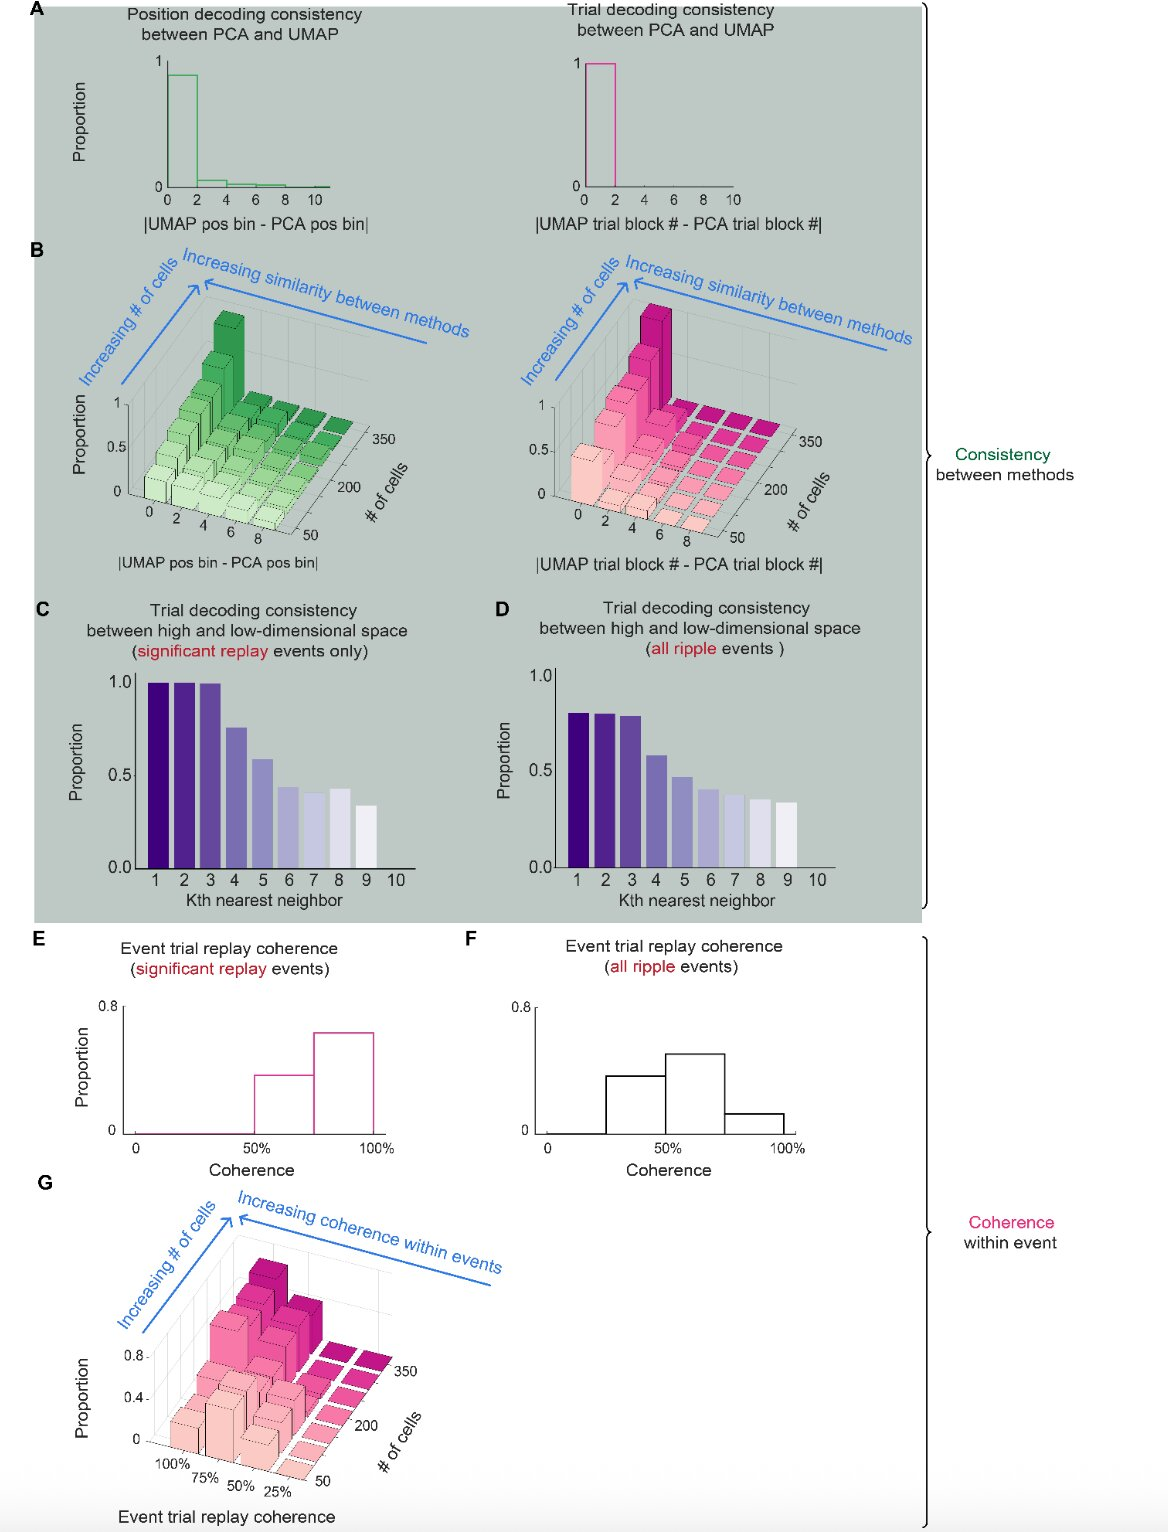
\includegraphics[width=\textwidth]{figures/ch_selection2024/Extended_Fig18.jpg}
\caption[Extended Data Fig.~18: Quantifying the decoding consistency between methods and within-event replay coherence]{\textbf{Extended Data Fig.~18: Quantifying the decoding consistency between methods and within-event replay coherence.}
(A) Consistency between UMAP and PCA decoding results, measured by the difference in decoding results from the two methods. Left, consistency between UMAP and PCA results for position decoding. Right, consistency between UMAP and PCA results for trial block decoding. 0 means PCA and UMAP decoded to the same position bin or trial block.
(B) Neurons used for the decoding analysis were downsampled. Left, consistency between UMAP and PCA for position decoding. Right, consistency between UMAP and PCA for trial block identity decoding.
(C) For all significant replay events, the consistency between the original high-dimensional and the reduced low-dimensional space was plotted. A data point was considered consistent if decoded trial block identities were the same in both spaces. For the first three nearest neighbors, the decoded trial block identity between the high and low-dimensional space was 100\% consistent.
(D) Similar to (C), but for all (not just significant) SPW-R events.
(E) Distribution of within-event coherency for significant replay events. The coherency of each event was measured as the proportion of time bins that share the same trial block label as the mode for that event.
(F) Similar to (E), but for all (not just significant) ripple events.
(G) As in (B), downsampling analysis with decreasing the number of neurons used for decoding was performed. More neurons included for decoding resulted in higher within-event trial replay coherency.}
\label{fig:selection2024-ext18}
\end{figure}

\begin{figure}[htbp]
\centering
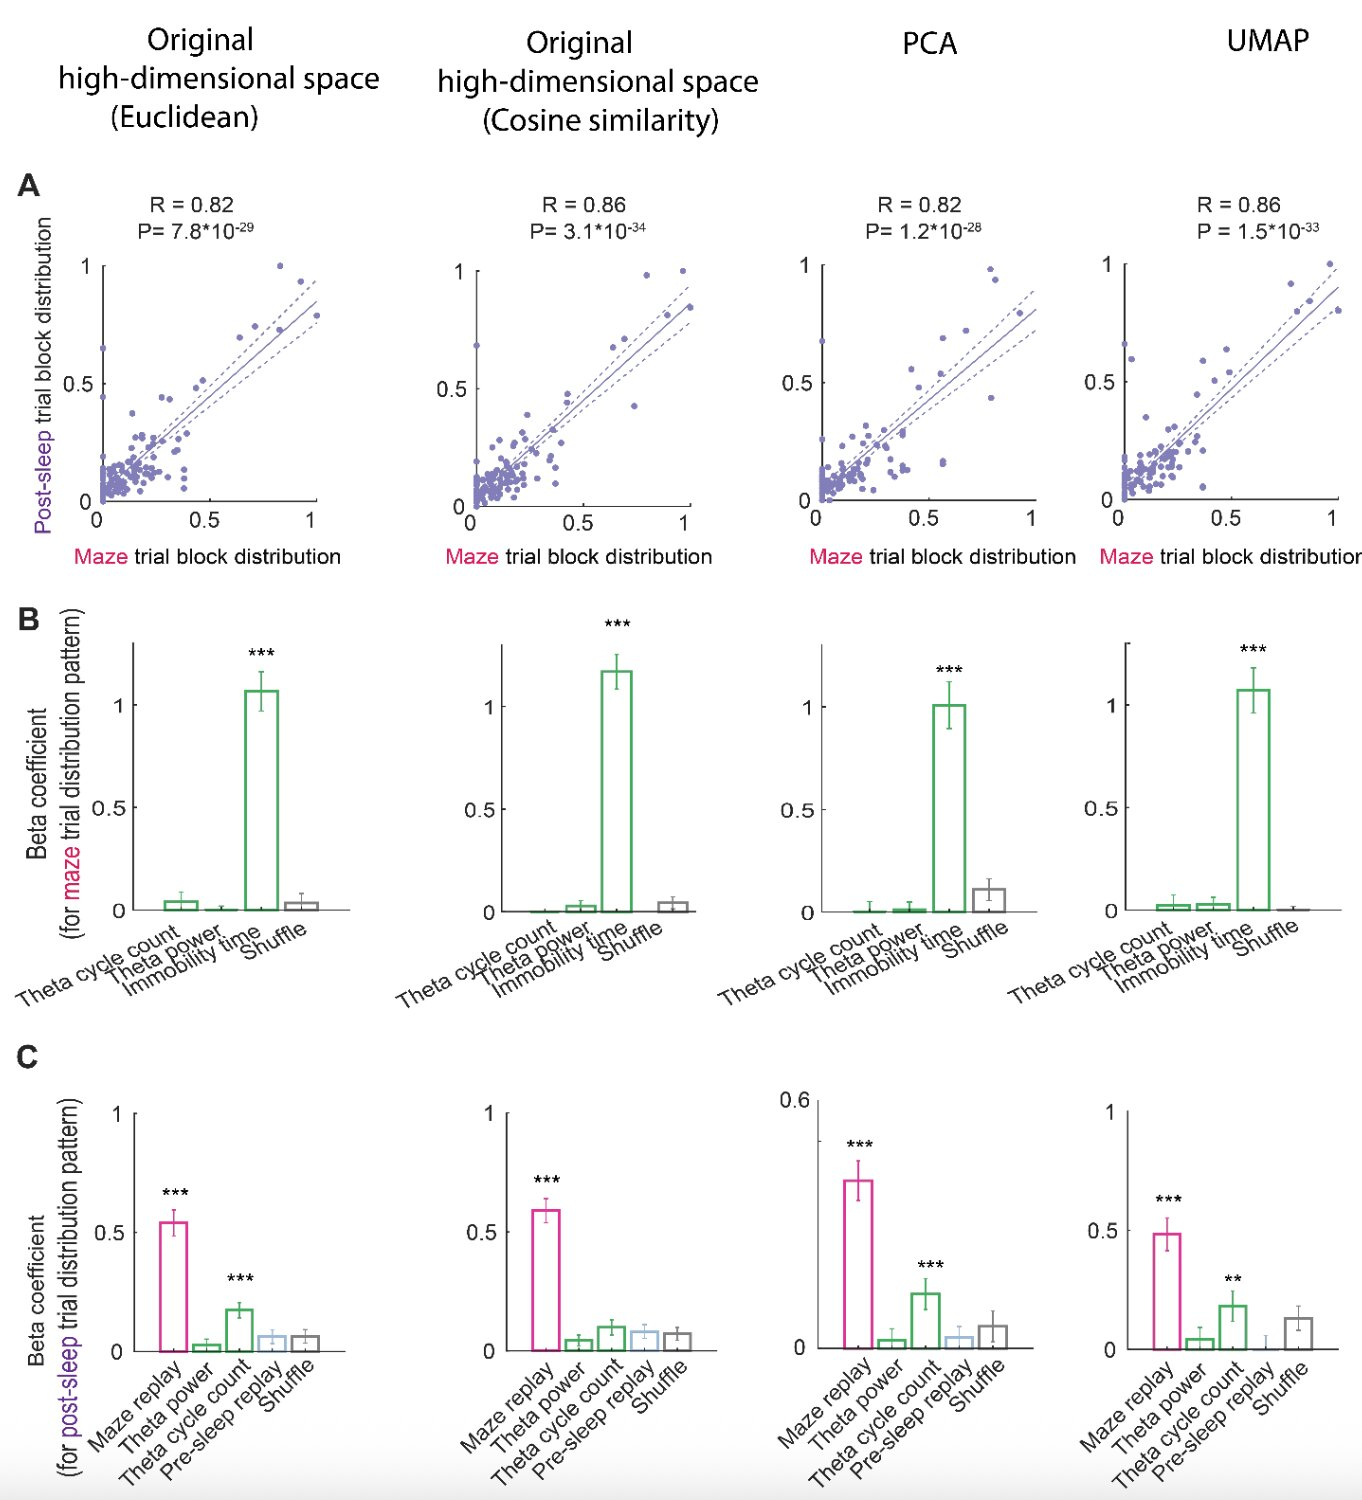
\includegraphics[width=\textwidth]{figures/ch_selection2024/Extended_Fig19.jpg}
\caption[Extended Data Fig.~19: Correlational and regression summary statistics are consistent across different methods]{\textbf{Extended Data Fig.~19: Correlational and regression summary statistics are consistent across different methods.}
(A) Correlation between maze replay events versus the post-experience sleep replay events, for their trial block distribution patterns. The results from four different decoding methods were presented in parallel to highlight the consistency across different methods.
(B) The predictive relationship between the trial block distribution pattern of maze replay events and other candidate variables, including the trial block distribution patterns of theta cycles, theta power and immobility time, and trial-shuffle data. For decoding from the original high-dimensional space with Euclidean distance metric, ***$P < 10^{-25}$ for immobility time; for decoding from high-dimensional space with cosine similarity, ***$P < 10^{-19}$ for immobility time; for PCA, ***$P < 10^{-16}$ for immobility time; for UMAP, ***$P < 10^{-5}$ for immobility time.
(C) The predictive relationship between trial block distribution pattern of post-experience sleep and other candidate variables. For decoding from original high-dimensional space with Euclidean distance metric, ***$P < 10^{-16}$ for awake replay, ***$P < 10^{-7}$ for theta cycle number; for decoding from high-dimensional space with cosine similarity, ***$P < 10^{-20}$ for awake replay; for PCA, ***$P < 10^{-12}$ for awake replay, ***$P < 10^{-6}$ for theta cycle number; for UMAP, ***$P < 10^{-10}$ for awake replay, **$P < 10^{-3}$ for theta cycle number. The relative predictive power of a given metric was considered non-significant when it overlapped with zero ($n = 16$ sessions from 5 animals).}
\label{fig:selection2024-ext19}
\end{figure}

\begin{figure}[htbp]
\centering
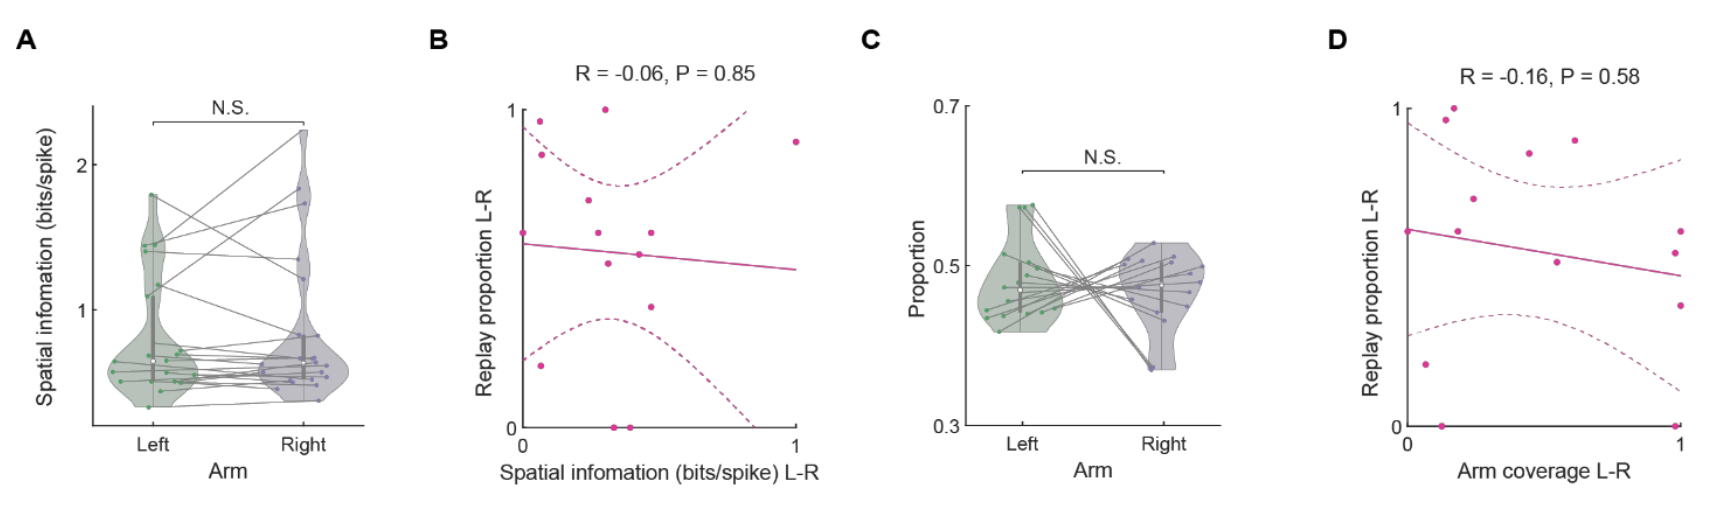
\includegraphics[width=\textwidth]{figures/ch_selection2024/Extended_Fig20.png}
\caption[Extended Data Fig.~20: Replay arm distribution pattern cannot be explained by the difference in decodability of the two side arms of the maze]{\textbf{Extended Data Fig.~20: Replay arm distribution pattern cannot be explained by the difference in decodability of the two side arms of the maze.}
(A) Mean spatial information for left versus right side arm segments. Each dot in the violin plot represents mean spatial information across all cells from one session (N.S. not significant, $P = 0.76$; unpaired t-test; $n = 13$ sessions from 5 animals).
(B) Correlation between spatial information difference and replay proportion difference between left and right arm. This shows that the difference in replay distribution across arms could not be explained by the difference in decodability (measured by the spatial information score) between the two arms (Pearson correlation coefficient, $R = 0.07$, $P = 0.85$; $n = 13$ sessions from 5 animals).
(C) Proportion of left versus right arm visit across sessions. Each dot in the violin plot represents one session (N.S. not significant; $P = 0.33$; unpaired t-test; $n = 13$ sessions from 5 animals).
(D) Correlation between the difference in arm visit and difference in replay proportion between left and right arm (Pearson correlation coefficient, $R = -0.16$, $P = 0.58$; $n = 13$ sessions from 5 animals).}
\label{fig:selection2024-ext20}
\end{figure}
